%\documentclass[a4paper,10pt]{article} % 11pt

\documentclass[a4paper,11pt]{article} % added Jan 3, 2021

%\documentclass[letterpaper,10pt]{article} % 10pt % comented Jan 3, 2021
%Use article for short documents
\usepackage[T1]{fontenc} % uncommented Jan 3, 2021
\usepackage{parskip}
\usepackage{latexsym,amsmath,amssymb}
%\usepackage{natbib}
\usepackage{graphicx}
\usepackage{times} % uncommented Jan 3, 2021
\usepackage{zi4}
\usepackage[letterpaper,left=4cm,right=4cm,top=3cm,bottom=3cm]{geometry}
%\usepackage[a4paper,left=4cm,right=4cm,top=3cm,bottom=3cm]{geometry}
\usepackage{float} % force figure
\usepackage{breakcites} % break citations between lines (prevent from flowing over)

\usepackage{hyperref} % hyperlinks
\usepackage[all]{hypcap}    %for going to the top of an image when a figure reference is clicked


\usepackage[nottoc,numbib]{tocbibind} % References in contents?


\pagestyle{myheadings} % page numbers on top right

\thispagestyle{empty}

\title{Normal linear Markov model with applications to polygenic inheritance}
\author{Jesse Murray}
\date{}

\begin{document}
\maketitle


\pagenumbering{arabic}



\section*{Abstract}
A Markov model of polygenic inheritance is proposed. Population members reproduce in discrete time, i.e., generations, and have phenotypic scores in continuous space. The initial condition is a population with a standard normal distribution of scores. Child scores relate to parent scores through a normal linear model, which is parametrized by a regression and residual coefficient. This simple formulation results in normal population distributions for all generations -- as expected, and normal conditional distributions for the scores of descendants and ancestors of any generation-gap $n$ apart. Furthermore, the parameters of these conditional distributions follow exponential functions of the generation gap, such that the conditional distributions converge to the population distribution as $n$ increases. That is, as the distance to a descendant or ancestor increases, predictive-ability is asymptotically lost with an exponential function. The regression and residual coefficients determine the rate constants of these exponential functions so that a robust measure of mobility -- also of information-loss -- is introduced as the ratio of the residual to the regression coefficient. Furthermore, the Markov process obtains a stationary distribution when the population variance is stable (constant) between generations, and when scores are indexed by percentile. Stationary distributions are reversible, meaning the model of inheritance behaves identically going forwards and backward in time. Probability kernels are introduced, which can make important predictions over any generation-gap and can be summarized by percentile transition matrices, which are bisymmetric. For every possible combination of percentile-groups, e.g. quintiles, these matrices show the probability that the $n$-gap ancestor or descendant of an individual in, say quintile A, is in quintile B. These probabilities are referred to as attributable and destined, respectively, and are equivalent in percentile transition matrices. The matrices enable visualizations of multi-generational regression towards the mean and the effects of the mobility measure. Matrices are also constructed from observed data, enabling comparisons to the model. From two large datasets on the heights of parents and their children, the proposed model is verified through statistical tests for the one-step transition, and the regression and residual coefficients are estimated.


\let\thefootnote\relax\footnotetext{jesse.murray@stats.ox.ac.uk, \indent github.com/jessebmurray/polygenic}


\newpage

% CONTENTS
\tableofcontents
\clearpage


%\section{Introduction}



%% MODEL FORMULATION %%
\section{Introduction and formulation of the model}

\subsection{Analogy to polygenic inheritance}
Polygenic inheritance occurs when a trait is determined by many genes -- in the range of hundreds or thousands. In general, the observed phenotypic scores of these traits are normally distributed, an effect of the central limit theorem \cite{rieger, lange_article}. That is, many genes act largely independent of one another -- and can have any unspecified distribution -- combine through an additive sum to determine phenotypes, resulting in a normal distribution \cite{lange_book}. 

One example of a polygenic trait is human stature, for which 697 variants have been identified at genome-wide significance, together explaining only one-fifth of the heritability of adult stature \cite{preece, wood}. Furthermore, stature has an observed normal distribution and normal linear models have been used to predict adult child height from parent height \cite{luo}. Normal linear models can be generalized over multiple generations in the form of a Markov process to reveal deeper results about polygenic inheritance and multi-generational mobility. 

\subsection{Markov process model of inheritance}

% COMPLETE DESCRIPTION

A Markov process is proposed that seeks to provide a basic model for the multi-generational dynamics of inheritance for a univariate polygenic trait (such as human stature). The proposed Markov process exists in discrete time $ i \in \{0, 1, 2,...\}$, where $i$ is the generation index (parent, child, grandchild, etc.); and continuous space $X_i \in \mathbb{R}$, where $X_i$ is the phenotypic score of the analogized univariate polygenic trait. The terms \emph{score} and \emph{state} are used interchangeably in reference to the phenotypic score. 

\begin{description}
\item [Convention] Let $Z$ refer to a generic standard normal $Z \sim \mathcal{N}(0, 1)$. The mentions of $Z$ throughout the text are used for explanatory purposes and they can be assumed to be unassociated with one another unless specified otherwise.
\item [Convention] Let the tilde symbol, e.g. $\tilde{\mu}_{i+n} \equiv \mathrm{E}(X_{i+n}|X_i)$, denote conditional parameters, such as conditional expectation and variance, that describe an upward or downward (conditional) transition distribution. That is, $\tilde{\mu}_{i+n}$ and $\tilde{\sigma}_{i+n}$ are the conditional expectation and standard deviation (SD), respectively, of state $X_{i+n}$ given state $X_i$. 
\item [Convention] Let the parameters $\mu_i$ and $\sigma_i$ be the expectation and SD, respectively, of the marginal (population) distribution of state $X_i$. 
\end{description}

The proposed Markov process can be entirely derived from: (1.) the initial condition and (2.) the one-step downward transition. 

\begin{enumerate}
\item The initial score is drawn from a standard normal distribution representing the scores of the initial generation: $X_0 \sim \mathcal{N}(0, 1)$. That is, $\mu_0 = 0$ and $\sigma_0 = 1$. A normally distributed univariate polygenic trait can be standardized to meet this condition. 

\item The conditional one-step downward transition, i.e., the score of a child, given the score of its parent, is also drawn from a normal distribution: $X_{i+1}|X_i \sim \mathcal{N}(\tilde{\mu}_{i+1}, \tilde{\sigma}_{i+1}^2)$.
$$X_{i+1}|X_i = \tilde{\mu}_{i+1} + \tilde{\sigma}_{i+1} Z$$ 

\begin{enumerate}
\item A child's score is proportional to the score of its parent, which is scaled by $r$ -- the \emph{regression coefficient}. In order for there to be regression towards the population mean, we require $0 < r < 1$. 
$$\tilde{\mu}_{i+1} = rX_i$$

\item While the expected child's score can be calculated from the score of its parent, there is a normally distributed residual about the expected child score that has a SD equal to the marginal SD of the parent generation ($\sigma_i$) scaled by $r_s$ -- the \emph{residual coefficient}. For the residual SD to be positive and a degenerate normal distribution avoided, we require $r_s > 0$.
$$\tilde{\sigma}_{i+1} = r_s \sigma_i$$
\end{enumerate}
\end{enumerate}

\subsubsection{Brief and complete description of the process}
As we have shown, the Markov process can be constructed from the equations for the initial condition and the one-step downward transition:
$$X_0 \sim \mathcal{N}(0, 1)$$
$$X_{i+1}|X_i = rX_i+ r_s\sigma_iZ$$
The latter equation contains the important coefficients $r$ and $r_s$, which have been named the regression coefficient and the residual coefficient, respectively. 

\subsubsection*{Note about standardization to measured values}
The distribution of the initial generation was set to $X_0 \sim \mathcal{N}(0, 1)$, and it was briefly mentioned that the phenotypic score of any univariate polygenic trait, e.g. stature, which is measured in centimeters, could be standardized to have mean zero and variance one. Due to this initial standardization, the scores of all generations are given in z-scores relative to the initial generation. Therefore, to obtain a score in terms of its measured units, e.g., centimeters, it is necessary only to shift and scale the score by the mean and SD, respectively, of the initial generation. 

When handling measured data, it may be the case that one has the measured mean and SD of some other generation besides the initial generation. In that case, it is worth noting that the mean of all generations is zero under this model. Furthermore, the SD of any generation can be easily calculated with $r$ and $r_s$ from the SD of any other generation.


\subsection*{Adjustment for uniform environmental effects}
It is worth remarking on the historical observation of human heights increasing between generations, which has been attributed to population-wide improvements in the environment for growth, in terms of nutrition and health \cite{bogin}. Previous studies have suggested that overall improvements in access to food, dietary diversification, sanitation, water, living standards, and decreasing exposure to disease are responsible for the secular increases in height occurring in the 19th and 20th centuries across many developed countries \cite{perkins}. 

As was discussed in the limitations section, the model proposed here does not describe the average movement of the population mean between generations as a result of external effects that would uniformly shift the conditional mean of each child. However, we can include these effects in the model without causing any problems. Here, we denote $c$ by the increase in height between generations.
$$X_{i+1}|X_i = r(X_i - \mu_i) + \mu_i + c+ \epsilon$$
$$\epsilon \sim \mathcal{N}(0, r_s^2 \sigma_i^2)$$
This equation shows how the one-step transition is follows a normal linear model (where the explanatory variable is normally distributed). Typically, $\mu_i$ is standardized to zero for the initial distribution.

Then, the change to our model is quite straightforward and can be given entirely by the uniform shift in the marginal population mean, which previously has been assumed to be zero. 
$$\mu_{i+n} = \mu_i + nc$$
$$\mu_{i-n} = \mu_i - nc$$
The $\mu_{i \pm n}$ adjustment would then need to be applied to the means of all conditional and marginal descendant and ancestor distributions (described later). 

Alternatively, if $c$ varies over time (given by the generation number), we get the following form for the adjustment:
$$\mu_{i+n} = \mu_i + \sum_{t = i+1}^{i+n} c(t)$$
$$\mu_{i-n} = \mu_i - \sum_{t = i-1}^{i-n} c(t)$$

Note that the convergences to the marginal distributions (described later) are not affected as the adjustment constant is added to both the marginal and conditional expectation, and thus cancels out when the two are compared. We have discussed how population-wide increases in average stature over generations have generally resulted from improved nutrition. Such effects can easily be included within the model if necessary, as long as they act uniformly on all children. This is shown to be the case in both the large population-based and historical Pearson datasets. 


% NORMAL LINEAR 
\subsection{Estimation of parameters through the normal linear model}

In this paper, the regression and residual parameters are estimated from one-step transition data -- the paired observations of same-sex parents and children -- with a normal linear model. When handling this data the parent and child scores are standardized to the sample mean and SD of the measured parent scores, to match the form of the model. 

The vector of coefficients for this model is then $\beta = (c, r)$, which is estimated through ordinary least squares. In other words, in a plot of parent versus child scores, the estimate for $c$ is the intercept and the estimate for $r$ is the slope of the regression line. Additionally, the unbiased estimate of $r_s$ is obtained from the residual sum of squares (RSS): $\sqrt{RSS / (n-p)}$, where $p = 2$. The regression and residual parameters can also be estimated by other conditional and descendant distributions described here as these also follow normal linear relationships.



% ASSUMPTIONS AND LIMITATIONS
\subsection{Summary of assumptions and limitations}

\subsubsection*{Assumptions}
\begin{enumerate}
\item Normality of the polygenic trait. This assumption is generally supported by the literature consensus on the effect of the central limit theorem for additive polygenic traits. The normality assumption has been widely been confirmed within the literature on human stature \cite{luo}.
\item Normal linear relationship between parent and child statures. That is, the linear regression form of the one-step downward transition has normally distributed residuals. This has been verified for human stature \cite{luo}.
\item Equal probability and degree of successful reproduction for all members of the population -- regardless of their score. In other words, no members of the population have more children than other members, and no natural selection occurs. 
\item Phenotypes are determined by the many small effects (leading to the normal distribution), as well as the potential for uniform effects on all members. That is, a uniform shift in phenotypic scores between generations.
\item Under stable population variance, the assumption that the conditional child distribution has an SD of $r_s \sigma_i$ (proportional to the marginal parent generation SD) is immaterial and could be simply given by $r_s$ (without any \emph{scaling}). That is, the assumption of scaling, implicit in the residual coefficient vanishes under stable population variance. 
\end{enumerate}

\subsubsection*{Limitations}
\begin{enumerate}
\item Marginal populations implicitly exist in discrete time and are non-overlapping.
\item Changes in population size are not modeled. 
\item Over many generations ($n$-step transitions for when $n$ is large), the model appears to be more appropriate under the condition of stable population variance. Otherwise, the population variance eventually expands to $\infty$ or shrinks to $0$, depending on whether $r^2 + r_s^2$ is greater than one or less than one, respectively. Nonetheless, it will be discussed how proposed calculations of attributable and destined probabilities are undistorted by unstable population variance.
\end{enumerate}



%% PROPERTIES %%
\section{Properties of the model}
\subsection{Marginal population distribution}
The unconditional (marginal) distribution of a score can be shown by induction and the theorem of the sum of independent normal random variables (rvs) to be given by $X_n \sim \mathcal{N}(0, \sigma_n^2)$, which can also be written:
$$X_n = \sigma_nZ$$

This occurs because the residuals of the one-step downward transition are normally distributed about the conditional expectation. If the residuals were not normally distributed, the population would depart from the normal distribution in the next generation.

\begin{description}
\item [Definition] Let $\sigma_i^2$ -- the \emph{population variance} -- refer to the marginal variance of $X_i$, i.e., without the knowledge of any past or future score $X_{j}$, with $j \neq i$. The population variance is shown to be related to the population variance of a previous generation. Likewise, the \emph{population variance} can be shown to always remain zero under the model. 
\end{description}

Then, for $Z_\alpha$, $Z_\beta$ iid standard normals, the marginal random state $X_{i+1}$ can be written in terms of the population variance of the previous state.
$$X_{i+1} = r\sigma_iZ_\alpha + r_s\sigma_iZ_\beta$$

\subsubsection*{Population variance}
From the equation for the marginal random state $X_{i+1}$, it can be shown that $\sigma_{i+1}^2$ has the following one-step relationship with the previous population variance:
$$\sigma_{i+1}^2 = (r^2+r_s^2)  \sigma_i^2$$
By induction, the population variance can be computed from a previous population variance for an arbitrary step-length:
$$\sigma_{i+n}^2 = (r^2+r_s^2)^n  \sigma_{i}^2$$



% COVARIANCE AND CORRELATION
\subsection{Covariance and correlation}
The regression coefficient relates to the covariance and correlation between the scores of an ancestor and its descendant. Recall that when $n = 1$, we are then describing parent and child. 
$$\mathrm{Cov}(X_{i+n}, X_i) = r^n \sigma_i^2$$
$$\mathrm{Corr}(X_{i+n}, X_i) = r^n \frac{\sigma_i}{\sigma_{i+n}}$$






% CONDITIONAL DESCENDANT DISTRIBUTION
\subsection{Conditional descendant distribution}

In describing the process, we gave the conditional one-step downward transition, which was the rv of a child's score as a function of its parent's score. However, we would like to have a general expression for the probability distribution of a descendant's score given its ancestor's score, for any number of generations $n$ separating the two. 

The conditional distribution $X_{i+n}|X_i$ can be shown to be normally distributed with the following expressions for $\mathrm{E}(X_{i+n}|X_i)$ and $\mathrm{Var}(X_{i+n}|X_i)$:

$$X_{i+n}|X_i \sim \mathcal{N}( \tilde{\mu}_{i+n}, \tilde{\sigma}_{i+n}^2)$$

$$\tilde{\mu}_{i+n} = r^nX_i$$

$$\tilde{\sigma}_{i+n}^2 = [(r^2+r_s^2)^n-r^{2n}] \sigma_i^2$$

The equation for conditional variance results from continually re-applying the one-step downward transition, which leads to the following equation for $X_{i+n}|X_i$:
$$X_{i+n}|X_i = r^nX_i + r_s\sigma_i \sum_{j=1}^{n}r^{n-j}(r^2+r_s^2)^{\frac{j-1}{2}}Z_j$$

It might appear that to obtain $\tilde{\sigma}_{i+n}^2$, we would need to make the unpleasant summation of the squared coefficients that multiply each $Z_j$. However, the earlier equation for population variance can be deployed, in which $r^nX_i$ is treated as a rv instead of as a constant. Then, the population variance is equal to the sum of marginal variance of $r^nX_i$ and $\tilde{\sigma}_{i+n}^2$.
%
$$\sigma_{i+n}^2 =  (r^2+r_s^2)^n  \sigma_{i}^2 =  r^{2n}\sigma_i^2 + \tilde{\sigma}_{i+n}^2$$
%
After rearranging and taking the square root, we obtain the equation for $\tilde{\sigma}_{i+n}$.

Our result is consistent with the following fact, which can be shown by induction to hold for all real numbers $a$,  $b$:
$$(a+b)^n - a^n = b \sum_{j=1}^{n}a^{n-j}(a+b)^{j-1}$$

In the section on the conditional ancestor distribution, we will show another way the conditional descendant distribution can be obtained.




%% DOWNWARD CONVERGENCE
\subsection{Exponential convergence of the conditional descendant distribution}

\subsubsection*{Convergence to the marginal distribution}
The conditional distribution of a descendant's score, given its ancestor's score $X_{i+n}|X_i \sim \mathcal{N}( \tilde{\mu}_{i+n}, \tilde{\sigma}_{i+n}^2)$ converges to its marginal population distribution of $X_{i+n}$ for large $n$.

Under regression towards the mean, we have $0 < r < 1$, for which we get the following convergence for large $n$:
$$r^n \rightarrow 0$$
This convergence affects the conditional expectation, which converges to the marginal (population) mean:
$$\tilde{\mu}_{i+n} = r^nX_i \rightarrow 0$$
Likewise, the convergence of $r^n$ affects the conditional variance $\mathrm{Var}(X_{i+n}|X_i)$, which can be written:
$$\tilde{\sigma}_{i+n}^2 = \sigma_{i+n}^2 - r^{2n} \sigma_i^2$$
This equation can perhaps more helpfully be written as a ratio:
$$\frac{\tilde{\sigma}_{i+n}^2}{\sigma_{i+n}^2} = 1 - (\frac{r^2}{r^2+r_s^2})^n$$
Recalling that the process required $r_s > 0$, we see that the conditional variance converges to the population variance for large $n$:
$$\tilde{\sigma}_{i+n}^2 \rightarrow \sigma_{i+n}^2$$

In summary, as $n \rightarrow \infty$:
$$X_{i+n}|X_i \rightarrow X_{i+n}$$

By the polygenic analogy, this result says that after many generations, a population member's descendants will have scores that become asymptotically indistinguishable from the marginal scores of the population. In other words, as more generations separate an ancestor and its descendant, the ancestor's score becomes asymptotically useless for predicting the descendant's score.


\subsubsection*{Role of the coefficients}
The rate at which the conditional descendant distribution converges to the population distribution is determined by the regression and residual coefficients. 

From the expressions for the downward convergence in expectation as well as in variance, we see that the more regression towards the mean there is (\emph{smaller $r$}), the faster the downward convergence to the marginal distribution. Likewise, the less regression towards the mean there is (\emph{larger $r$}), the slower the downward convergence to the marginal distribution. 

From the expression for the downward convergence in variance, we that the less residual variance there is (\emph{smaller $r_s$}), the slower the convergence to the marginal distribution. That is, as long as $|r| < 1$, otherwise, the conditional expectation will not converge to $0$. Likewise, the larger the residual variance (\emph{larger $r_s$}), the faster the convergence to the marginal distribution. 


\subsubsection*{Degenerate lower bound for the residual coefficient}
We can show that $r \geq r^2 + r_s^2$ is essentially degenerate, resulting in a lower bound on $r_s$:
$$r_s > \sqrt{r(1-r)}$$

The possible values for $r$ and $r_s$ due to their initial requirements and this newly given lower bound on $r_s$ are shown in Figure \ref{fig:possible_r_rs}. 

\begin{figure}[h]
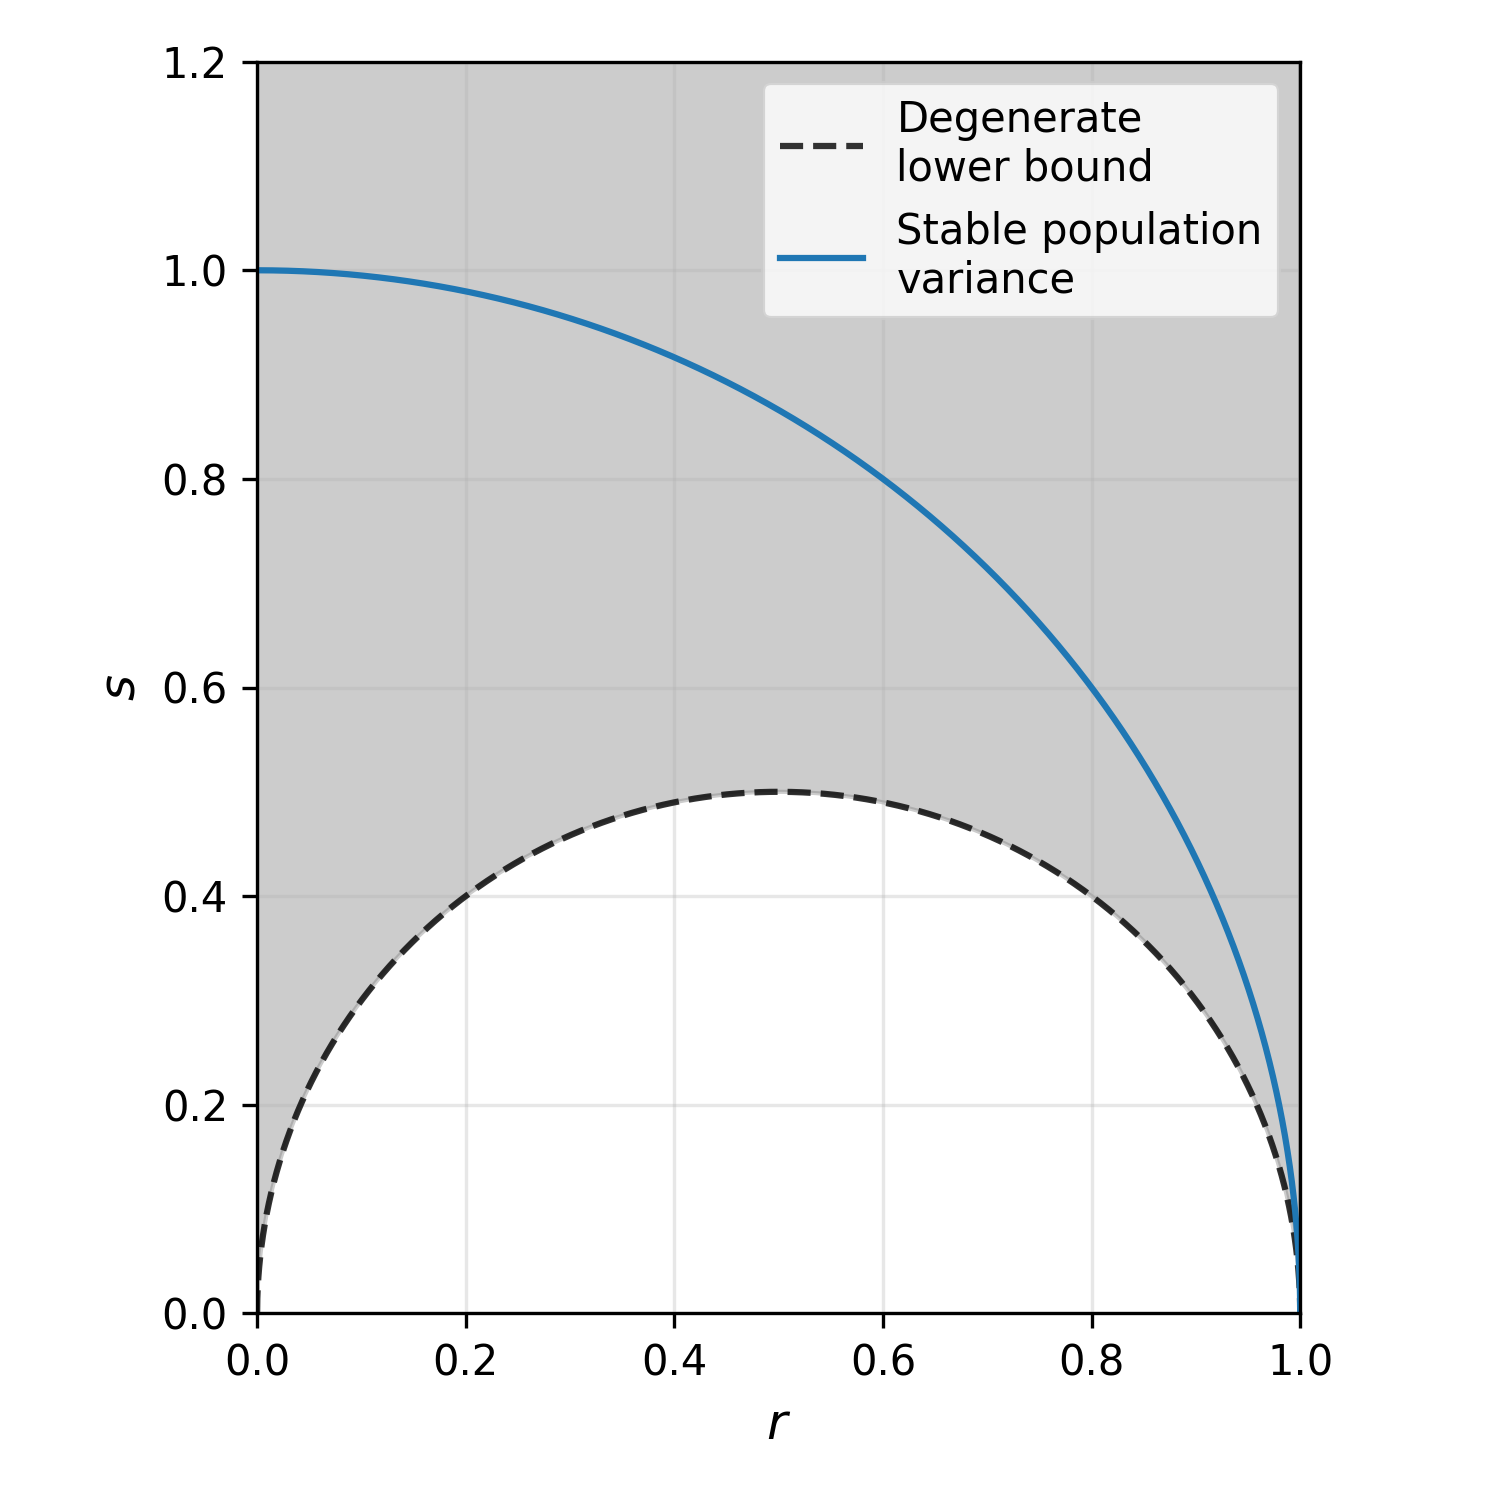
\includegraphics[width=3in]{figures/possible_r_rs.png}
\centering
\caption{Possible values for the regression and residual coefficients are given by the shaded area, which extends upwards for $r_s \rightarrow \infty$. The degenerate lower bound has $r_s > \sqrt{r(1-r)}$ and stable population variance (the stationary distribution) has $r_s = \sqrt{1-r^2}$.}
\label{fig:possible_r_rs}
\end{figure}

We can show why breaching this lower bound is degenerate by breaking up $r \geq r^2 + r_s^2$ into two cases.

In the first case: $r = r^2 + r_s^2$, then we have no regression to the mean relative to the population variances. In other words, all ancestors have the same expected z-score.
$$\frac{\tilde{\mu}_{i+n}}{\sigma_{i+n}^2} = \frac{X_i}{\sigma_i^2}$$


In the second case: $r > r^2 + r_s^2$, then we have $r^2 + r_s^2 < 1$ and $\sigma_{i+n}^2 \rightarrow 0$ for large $n$, as we have previously shown. While this is otherwise alright, here it leads to the variance of the marginal population shrinking to zero faster than the conditional expectation does, which causes the descendant's expected z-score to diverge.
$$\frac{\tilde{\sigma}_{i+n}^2}{\sigma_{i+n}^2} = (\frac{r}{r^2+r_s^2})^n \frac{X_i}{\sigma_i^2} \rightarrow \infty$$
As $X_i$ was arbitrary, all descendants' expected z-scores would diverge regardless of their ancestors' scores, which can be considered degenerate. 


\subsubsection*{Exponential functions for conditional expectation and variance}

The role of the coefficients can also be seen in the equations for the rate of change in the parameters of the conditional descendant distribution.

The rate of change in the conditional expectation is negative and increasing with $n$ (positive second partial derivative). Therefore, the conditional expectation asymptotically approaches zero, and the smaller $r$ is, the larger the negative rate. The natural logarithm is denoted by '$\log$'.
$$\frac{\partial }{\partial n}[\tilde{\mu}_{i+n}] = -\log(\frac{1}{r}) \, \tilde{\mu}_{i+n}$$


Likewise, the rate of change in the ratio of the conditional variance to the marginal variance is positive and decreasing with $n$ (negative second partial derivative). Therefore, the ratio asymptotically approaches one. The smaller $r$ is, or the larger $r_s$ is, the larger the positive rate of convergence.
$$\frac{\partial }{\partial n}[\frac{\tilde{\sigma}_{i+n}^2}{\sigma_{i+n}^2}] = \log(1+\frac{r_s^2}{r^2}) \, [1 - \frac{\tilde{\sigma}_{i+n}^2}{\sigma_{i+n}^2}]$$

We then get the following exponential functions:
$$\tilde{\mu}_{i+n} = X_i \, \exp[-\log(\frac{1}{r}) \, n]$$
$$\tilde{\sigma}_{i+n}^2 = \sigma_{i+n}^2 \, (1 - \exp[-\log(1+\frac{r_s^2}{r^2}) \, n])$$

Earlier, we derived the conditional distribution of the score of a descendant, given the score of its ancestor $X_{i+n}|X_i \sim \mathcal{N}( \tilde{\mu}_{i+n}, \tilde{\sigma}_{i+n}^2)$. Now we have just shown that the parameters of this distribution are both exponential functions of the generation gap $n$, and that both converge on the marginal parameters. In other words, the conditional expectation of a descendant's score exponentially approaches the population mean, and the conditional variance of a descendant's score also exponentially approaches the population variance. 




% POPULATION VARIANCE
\subsection{Population variance dynamics}

\subsubsection*{Unstable population variance}
We have shown that:
$$\sigma_{i+n}^2 = (r^2+r_s^2)^n  \sigma_{i}^2$$

Taking the limit $n \rightarrow \infty$: 
\begin{itemize}
\item For $r^2+r_s^2 < 1$ we have $\sigma_{i+n}^2 \rightarrow 0$.
\item For  $r^2+r_s^2 > 1$, we have $\sigma_{i+n}^2 \rightarrow \infty$. 
\end{itemize}

These degenerate limits could be prevented if $r$ or $r_s$ were inversely proportional to some power of the population variance $\sigma_i^2$. However, this negative feedback is not explored here. Instead, we discuss the simplest resolution to population variance instability, which is that $r^2+r_s^2 = 1$. Then, every generation has the same population variance.

\subsubsection*{Stable population variance}
We are particularly interested in the case where the population variance remains constant between generations. This would model a population in which the phenotypes of the polygenic trait do not become increasingly or decreasingly spread out between successive generations. 
$$\sigma_{i+1}^2 = \sigma_i^2$$
This occurs if and only if:
$$r^2+r_s^2 = 1$$
%
By induction, the population variance of any arbitrary generation $i$ is equal to the initial variance. 
$$\sigma_i^2 = 1$$



% STATIONARY DISTRIBUTION
\subsection{Stationary distribution}

\subsubsection*{Stable population variance implies stationary distribution}
It can be shown that the process is at a stationary distribution when there is stable population variance:
$$X_i \sim \mathcal{N}(0, 1)$$
$$X_{i+1} = r Z_\alpha + r_s Z_\beta$$
$$X_{i+1} \sim \mathcal{N}(0, r^2+r_s^2)$$
$$X_{i+1} \sim \mathcal{N}(0, 1)$$

\subsubsection*{Stationary distribution is reversible}
It will be shown in the section on the conditional ancestor distribution that the process behaves identically going forwards and backward in time when there is stable population variance.

\subsubsection*{Convergence to the stationary distribution}

From the downward convergence to the marginal distribution and the fact that the stationary distribution is reversible, it follows that the conditional ancestor distribution converges to the marginal distribution. 
As $n \rightarrow \infty$:
$$X_{i-n}|X_i \rightarrow \mathcal{N}(0, 1)$$



%% CONDITIONAL ANCESTOR DISTRIBUTION %%
\subsection{Conditional ancestor distribution}

Up until this point, we have only discussed the conditional rv of a descendant's score given its ancestor's score. We would however like to be able to describe the upward relationship: the probability distribution of an ancestor's score given its descendant's score, for any number of generations $n$ separating the two. 

\begin{description}
\item [Convention] In order to remain consistent with our earlier notation, it will be easiest to think of the generation number of the ancestor as also $b = i - n$. That is, the ancestor existed at time $b$, which is $n$ generations \emph{before} the current time $i$. 
\end{description}

One way to obtain the distribution of $X_{i-n}|X_i$ is with Bayes' rule. 
$$f(x_{i-n}|x_i) \propto f(x_{b+n}|x_b) f(x_b)$$
This is similar, though not identical, to finding the posterior distribution for $\mu$ of a normal distribution when the prior distribution for $\mu$ is normal. Then, a normal prior times the normal likelihood gives a normal posterior. However, because $X_{b+n}|X_b \sim \mathcal{N}(r^n X_b, \tilde{\sigma}_{b+n}^2)$, such that the $r^n$ term obfuscates the conjugate prior, this approach requires unpleasant algebra for completing the square in the exponent. 

An alternative approach is to recognize that $X_{i-n}$ and $X_i$ form a bivariate normal distribution. Then, the conditional distribution of $X_{i-n}$ given $X_i$ must be normally distributed with the following parameters:
$$\mathrm{E}(X_{i-n}|X_i) = \mathrm{E}(X_{i-n}) + \frac{\mathrm{Cov}(X_{i-n}, X_i)}{\mathrm{Var}(X_i)}[X_i - \mathrm{E}(X_i)]$$
$$\mathrm{Var}(X_{i-n}|X_i) = \mathrm{Var}(X_{i-n}) - \frac{[\mathrm{Cov}(X_{i-n}, X_i)]^2}{\mathrm{Var}(X_i)}$$

Using our earlier results and simplifying, we get that the conditional distribution $X_{i-n}|X_i$ is normally distributed with the following expressions for $\mathrm{E}(X_{i-n}|X_i)$ and $\mathrm{Var}(X_{i-n}|X_i)$:

$$X_{i-n}|X_i \sim \mathcal{N}( \tilde{\mu}_{i-n}, \tilde{\sigma}_{i-n}^2)$$

$$\tilde{\mu}_{i-n} = (\frac{r}{r^2+r_s^2})^n X_i$$

$$\tilde{\sigma}_{i-n}^2 = [1 - (\frac{r^2}{r^2+r_s^2})^n] \sigma_{i-n}^2$$

The bivariate normal approach can also be used to confirm our earlier expressions for $\tilde{\mu}_{i+n}$ and $\tilde{\sigma}_{i+n}^2$, which were previously obtained by continually re-applying the one-step downward transition of the Markov process.

\subsubsection*{One-step upward transition}
The one-step upward transition describes the conditional distribution of a parent's score given its child's score. We can show that $X_{i-1}|X_i \sim \mathcal{N}( \tilde{\mu}_{i-1}, \tilde{\sigma}_{i-1}^2)$ with the following parameters:
$$\tilde{\mu}_{i-1} = \frac{r}{r^2+r_s^2} X_i$$
$$\tilde{\sigma}_{i-1}^2 = \frac{r_s^2}{r^2+r_s^2} \sigma_i^2$$

This has a very similar form to the one-step downward transition, only the coefficients have changed slightly.
$$X_{i-1} = \frac{r}{r^2+r_s^2} X_i + \frac{r_s}{\sqrt{r^2+r_s^2}} \sigma_{i} Z$$


\subsubsection*{Stationary distribution is reversible}

Because we have $r^2+r_s^2 = 1$ under stable population variance, ie., the stationary distribution, the process behaves the same way going forwards and backwards in time:
$$X_{i-1} = r X_i + r_s \sigma_{i} Z$$
It is straightforward to show that $X_{i-n}|X_i \sim \mathcal{N}( \tilde{\mu}_{i-n}, \tilde{\sigma}_{i-n}^2)$ has the same form as $X_{i+n}|X_i \sim \mathcal{N}( \tilde{\mu}_{i+n}, \tilde{\sigma}_{i+n}^2)$ under the stationary distribution:
$$\tilde{\mu}_{i-n} = \tilde{\mu}_{i+n} = r^nX_i$$
$$\tilde{\sigma}_{i-n}^2 = \tilde{\sigma}_{i+n}^2 = 1-r^{2n}$$





% UPWARD CONVERGENCE
\subsection{Exponential convergence of the conditional ancestor distribution}

\subsubsection*{Convergence to the marginal distribution}
The conditional distribution of an ancestor's score, given its descendant's score $X_{i-n}|X_i \sim \mathcal{N}( \tilde{\mu}_{i-n}, \tilde{\sigma}_{i-n}^2)$ converges to the marginal population distribution of $X_{i-n}$ for large $n$.

Then, for large $n$, we have the following convergences:
$$(\frac{r}{r^2+r_s^2})^n \rightarrow 0$$
$$(\frac{r^2}{r^2+r_s^2})^n \rightarrow 0$$

Therefore, we have convergence both in conditional expectation and variance:
$$\tilde{\mu}_{i-n} \rightarrow 0$$
$$\tilde{\sigma}_{i-n}^2 \rightarrow \sigma_{i-n}^2$$
In summary, as $n \rightarrow \infty$:
$$X_{i-n}|X_i \rightarrow X_{i-n}$$

We have thus confirmed our earlier stated lower bound on $r_s$, as the upward conditional expectation would not converge under the degenerate condition.


\subsubsection*{Role of the coefficients}
The rate at which the conditional ancestor distribution converges to the population distribution is determined by the regression and residual coefficients. 

It is worth noting that the ratio of the downward conditional variance to the marginal variance is the same as the ratio of the upward conditional variance to the marginal variance, shown earlier. Therefore, the effects of $r$ and $r_s$ are the same for both the upward and downward convergence of conditional variance to the marginal variance.

From the expressions of convergence for both expectation and variance, we see that a smaller regression coefficient $r$ leads to faster convergence, and vice versa; and that a smaller residual coefficient $r_s$ leads to slower convergence, and vice versa. Unlike for the downward convergence, upward convergence does not require $|r| < 1$.

\subsubsection*{Exponential functions for conditional expectation and variance}
The role of the coefficients can also be seen in the equations for the rate of change in the parameters of the conditional ancestor distribution.

The rate of change in the conditional expectation is negative and increasing with $n$ (positive second partial derivative). Therefore, the conditional expectation asymptotically approaches $0$. The smaller $r$ is, or the larger $r_s$ is, the larger the negative rate. 
$$\frac{\partial}{\partial n}[\tilde{\mu}_{i-n}] = -\log(\frac{r^2 + r_s^2}{r}) \, \tilde{\mu}_{i-n}$$

The rate of change in the ratio of the conditional variance to the marginal variance has the same form as in the upward convergence. Therefore, the rate of change is positive and decreasing with $n$ (negative second partial derivative), asymptotically approaching one. The smaller $r$ is, or the larger $r_s$ is, the larger the positive rate of convergence.
$$\frac{\partial }{\partial n}[\frac{\tilde{\sigma}_{i-n}^2}{\sigma_{i-n}^2}] = \log(1+\frac{r_s^2}{r^2}) \, [1 - \frac{\tilde{\sigma}_{i-n}^2}{\sigma_{i-n}^2}]$$

We then get the following exponential functions:
$$\tilde{\mu}_{i-n} = X_i \, \exp[-\log(\frac{r^2 + r_s^2}{r}) \, n]$$
$$\tilde{\sigma}_{i-n}^2 = \sigma_{i-n}^2 \, (1 - \exp[-\log(1+\frac{r_s^2}{r^2}) \, n])$$

Earlier, we derived the conditional distribution of the score of an ancestor, given the score of its descendant $X_{i-n}|X_i \sim \mathcal{N}( \tilde{\mu}_{i-n}, \tilde{\sigma}_{i-n}^2)$. Now we have just shown that the parameters of this distribution are both exponential functions of the generation gap $n$, and that both converge on the marginal parameters. In other words, the conditional expectation of an ancestor's score exponentially approaches the population mean, and the conditional variance of an ancestor's score also exponentially approaches the population variance. 









%% MODEL VERIFICATION FOR HUMAN STATURE %%
\section{Application to human stature}

The model formulation is checked against data on the heights of parents and their adult children. Because all of the properties of the Markov process follow from the initial condition and the one-step downward transition, confirming their accuracy confirms the model's properties over any number of steps.

\subsubsection*{Verifying the model}
We consider the parental generation to be the initial generation. Then, we have two basic requirements to confirm our model:
\begin{enumerate}
\item The parental heights are modeled by the initial condition.
\item The conditional distribution of the child heights is modeled by the one-step downward transition, for which we can also refer to its linear regression form.
\end{enumerate}



\subsection{Large population-based study}

The study \emph{Target Height as Predicted by Parental Heights in a Population-Based Study}, published in \emph{Nature -- Pediatric Research} \cite{luo}, analyzed the relationship between the heights of adult children and the heights of their parents for predicting target height. The data they analyzed was from a large sample ($n$ = 2402) of normal Swedish children born in the 1970s. 


\subsubsection*{The initial condition}
Unfortunately, the authors did not report on the normality of the parental heights in the dataset. Nonetheless, the authors cite a paper that reports height to be normally distributed in a population \cite{preece}. Thus, we can assume that the parental heights were normally distributed, confirming the initial condition.


\subsubsection*{The one-step downward transition}

An increase in height between generations was observed, amounting to 0.7 cm for male and 1.0 cm for female subjects. We have shown that as long as the increase is uniform, i.e., not dependent on the parent's score, then we can include the increase in the model by the addition of a constant-term in the linear regression. That is, as long as the mean residual values are zero over all possible parent scores, then the increase is uniform and is accurately described by the adjustment to the model.

The authors tested the validity of a normal linear model for the one-step transition of parent to child heights. Their model was identical to the linear regression form of the one-step transition discussed earlier. The authors confirm the veracity of the linear model, and thus they confirm the formulation of the one-step downward transition.

The authors confirm the validity of the normal linear model by the following tests:
\begin{enumerate}
\item The residuals were normally distributed (tested by skewness and kurtosis).
\item The mean residual values were fairly constant over the range of midparental heights, fluctuating around zero, and were only statistically significantly above zero ($p < 0.05$) for very short mid-parental heights (below $-2$ SDs).
\item The mean residual values were constant over the range of difference in parental heights.
\item The residual SDs were constant over the range of midparental height  
\item The residual SDs were constant over the range of difference in parental heights.
\end{enumerate}

In summary, the residuals were normally distributed about the linearly predicted child height, and neither midparental height nor the difference in parental height affected the residual values. In terms of the model, this result means that both $r$ and $r_s$ are neither dependent on $X_i$ nor the difference between $X_i$ and the score of the mating partner. 

The authors also conclude that the predictive accuracy was also not affected by assortative mating, as they observed a correlation coefficient between the parents of 0.27, which is an indication of assortative mating.



\subsubsection*{Observed coefficients}
Varied values of $r$ and $r_s$ were found for using mothers' heights to predict sons' heights, fathers' heights to predict sons' heights, mothers' heights to predict daughters' heights, etc. However, these four possibilities averaged around $r$ = 0.49 and $r_s$ = 0.88, which essentially produces stable population variance, giving a ratio of the adult children's SD to the parents' SD, which we will from now on call the SD ratio, of 1.01.
$$\mathrm{SD} \, \mathrm{ratio} = \frac{\sigma_{i+1}}{\sigma_i}$$

\subsubsection*{Model can be completely confirmed for stable population variance}
From one-step transition data, we cannot confirm the part of our model that says $\tilde{\sigma}_{i+1} = r_s \sigma_i$, that is, except for when there is stable population variance. Then, $\sigma_i$ is constant, and we have $\tilde{\sigma}_{i+1} = r_s$, because the initial variance is standardized to one.

In the dataset, the observed ratio of the sons-fathers SD ratio was 0.978, consistent with stable population variance. The observed ratio of the daughters-mothers SD ratio was 1.16, somewhat consistent with stable population variance. 

Members towards the outer edges of the population distribution of stature may be less likely to have children -- or have fewer children -- than those towards the middle, which would have the effect of counteracting otherwise expanding population variance. On the other hand, if this is not observed, then it is reasonable to assume that the stable population variance condition applies to human stature, in which case the resultant stationary distribution and all of its properties apply as well. 



\subsection{Pearson dataset}

Karl Pearson organized the collection of data on over 1,100 families in England in the 1890s. The dataset he collected contains the heights of mothers, fathers and their adult children with no more than two adult children per family \cite{pearson}. All the adult children were at least age 18, and all of the parents were at most 65 years of age. Here, we check the validity of the model by verifying the initial condition and the one-step downward transition. We present this in detail for the daughter-mother data ($n$ = 1375) with statistical tests at the 5\% level.


\subsubsection*{The initial condition}

It is obvious from the Q-Q plot in Figure \ref{fig:qq_pearson_x} that the mother's scores are normally distributed. Furthermore, the normality assumption passes statistical tests of skewness and kurtosis, as well as D’Agostino and Pearson's test that combines skew and kurtosis to produce a single test of normality.

\begin{figure}[h]
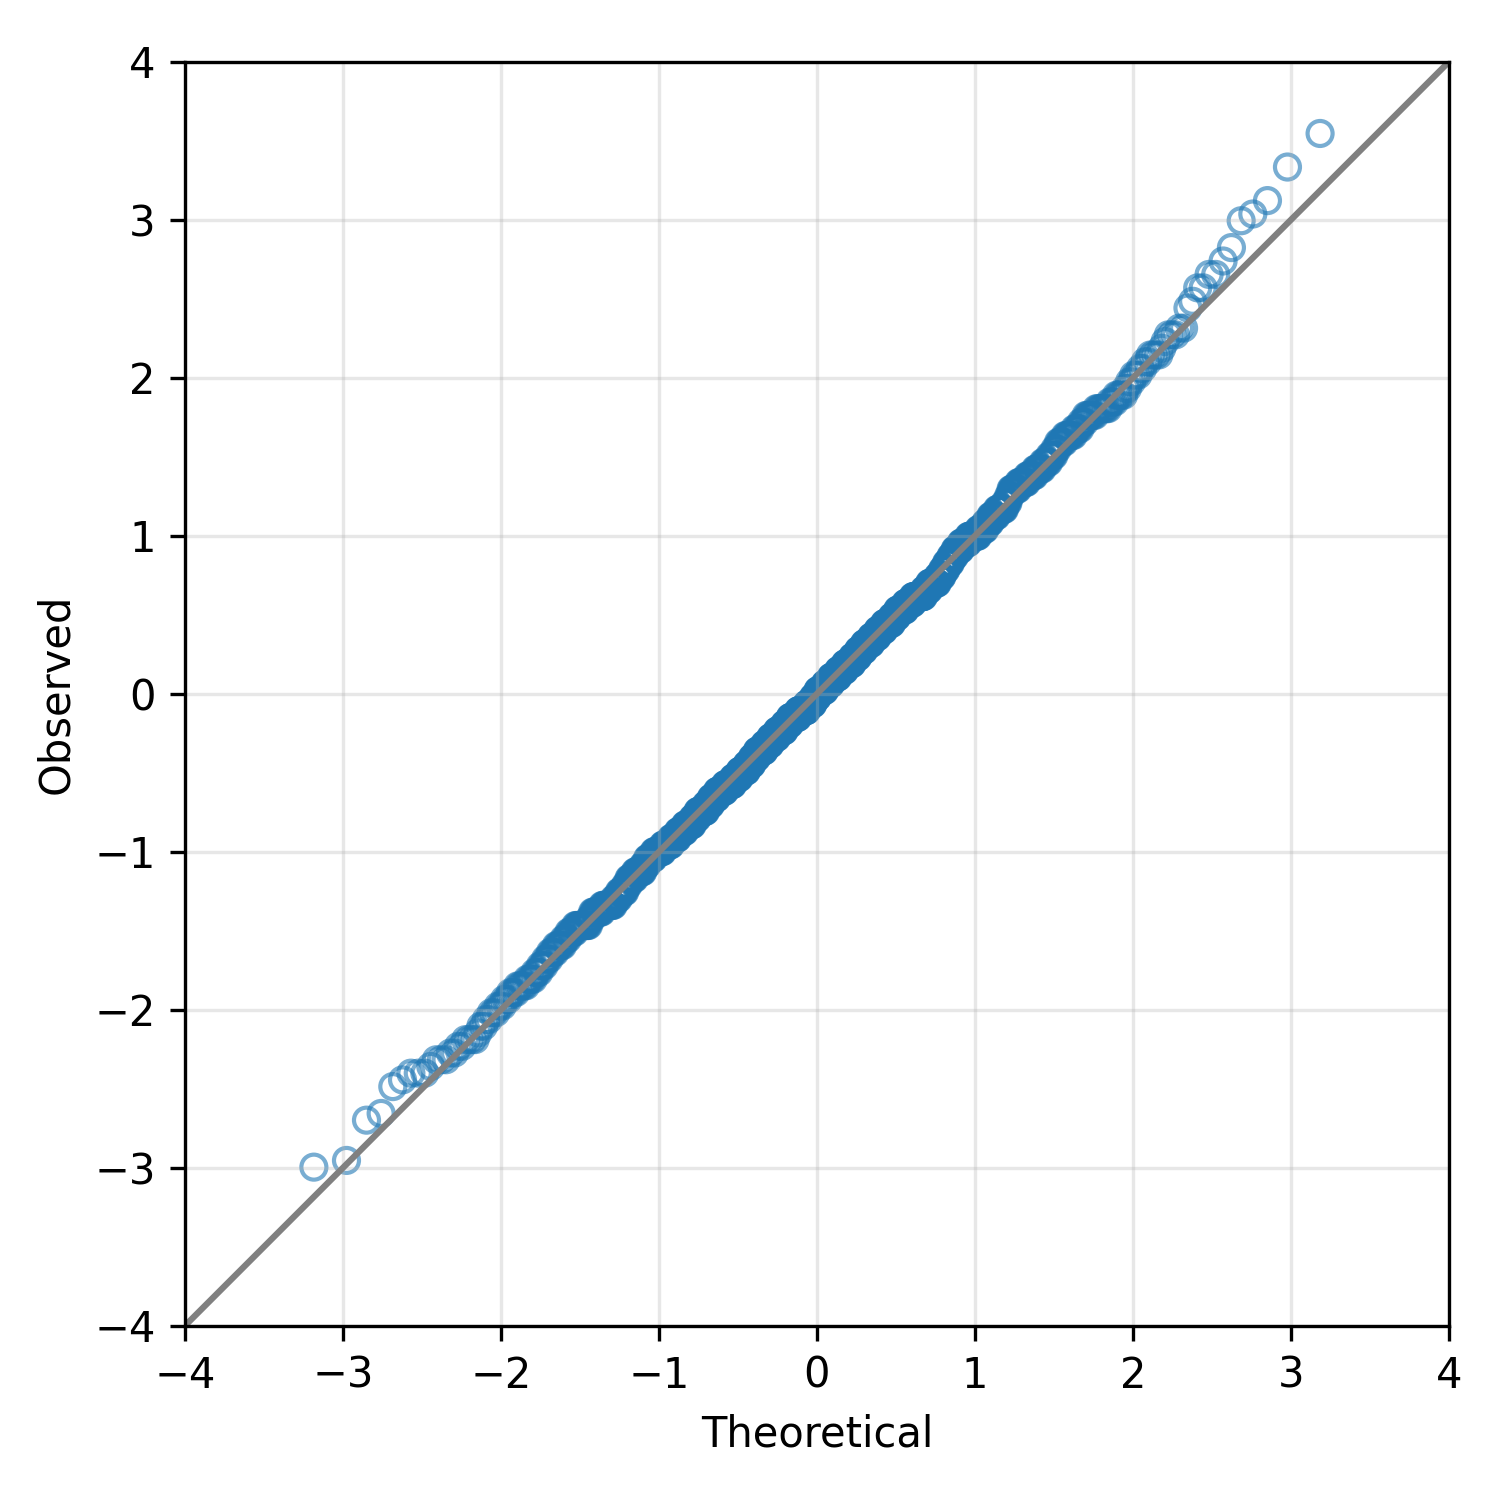
\includegraphics[width=3in]{figures/pearson-lee-mother-daughter-qq_parents.png}
\centering
\caption{Q-Q plot of the mothers' scores in the Pearson female dataset.}
\label{fig:qq_pearson_x}
\end{figure}


\subsubsection*{The one-step downward transition}

As in the Swedish data, an increase in height between generations was observed, amounting to 3.3 cm, meaning that the adjustment to our model must be made. 

We can see that the residuals were normally distributed from the Q-Q plot in Figure \ref{fig:qq_pearson_epsi}. Furthermore, the normality assumption passes statistical tests of skewness, kurtosis, and D’Agostino and Pearson's test.

Likewise, we can show in Figure \ref{fig:pearson_residuals_by_score} that residuals are uncorrelated with the parent scores. This means that the adjustment constant can be applied safely as the shift applies uniformly to all children. 


\begin{figure}[p]
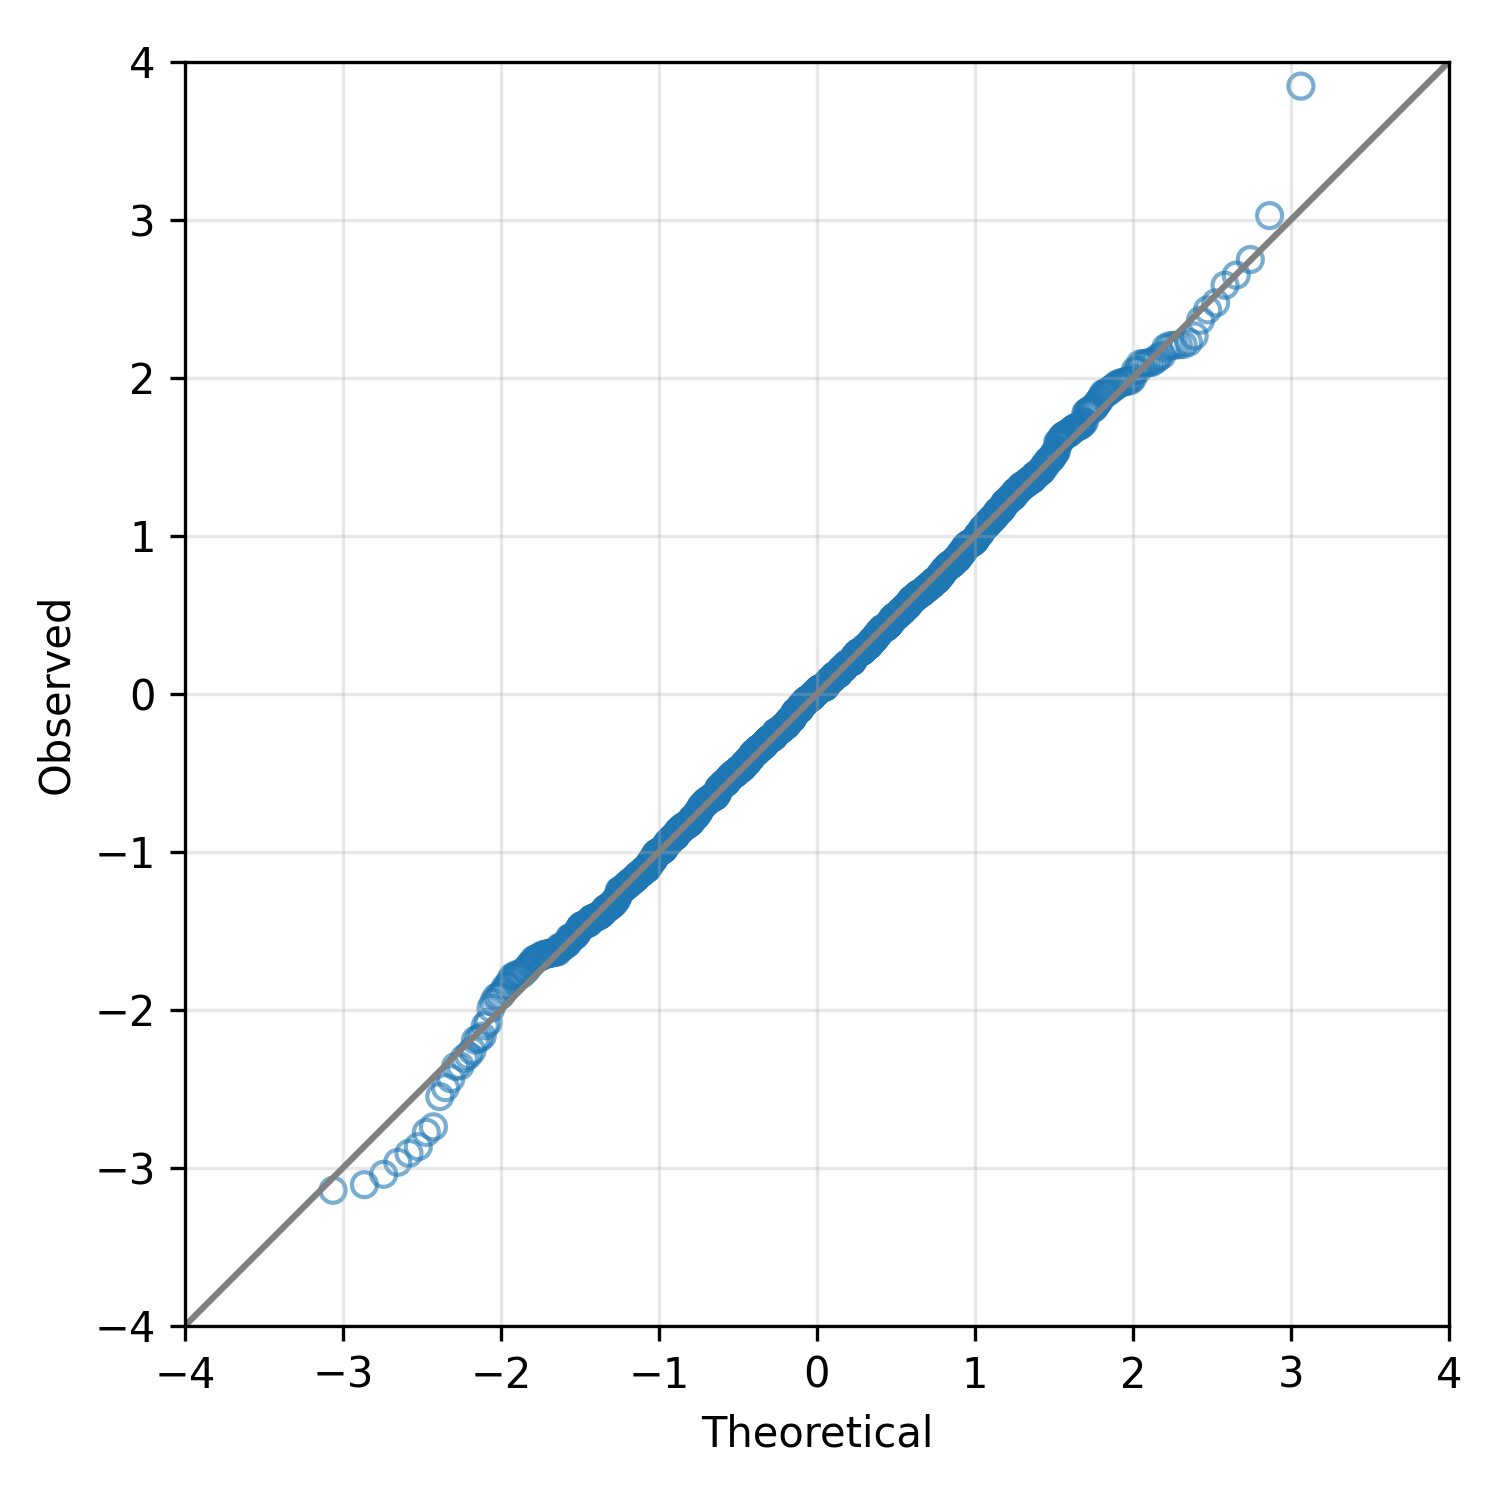
\includegraphics[width=3in]{figures/pearson-lee-mother-daughter-qq_residuals.png}
\centering
\caption{Q-Q plot of the daughters' residuals in the Pearson female dataset.}
\label{fig:qq_pearson_epsi}
%\end{figure}

\vspace{2cm}

%\begin{figure}[h]
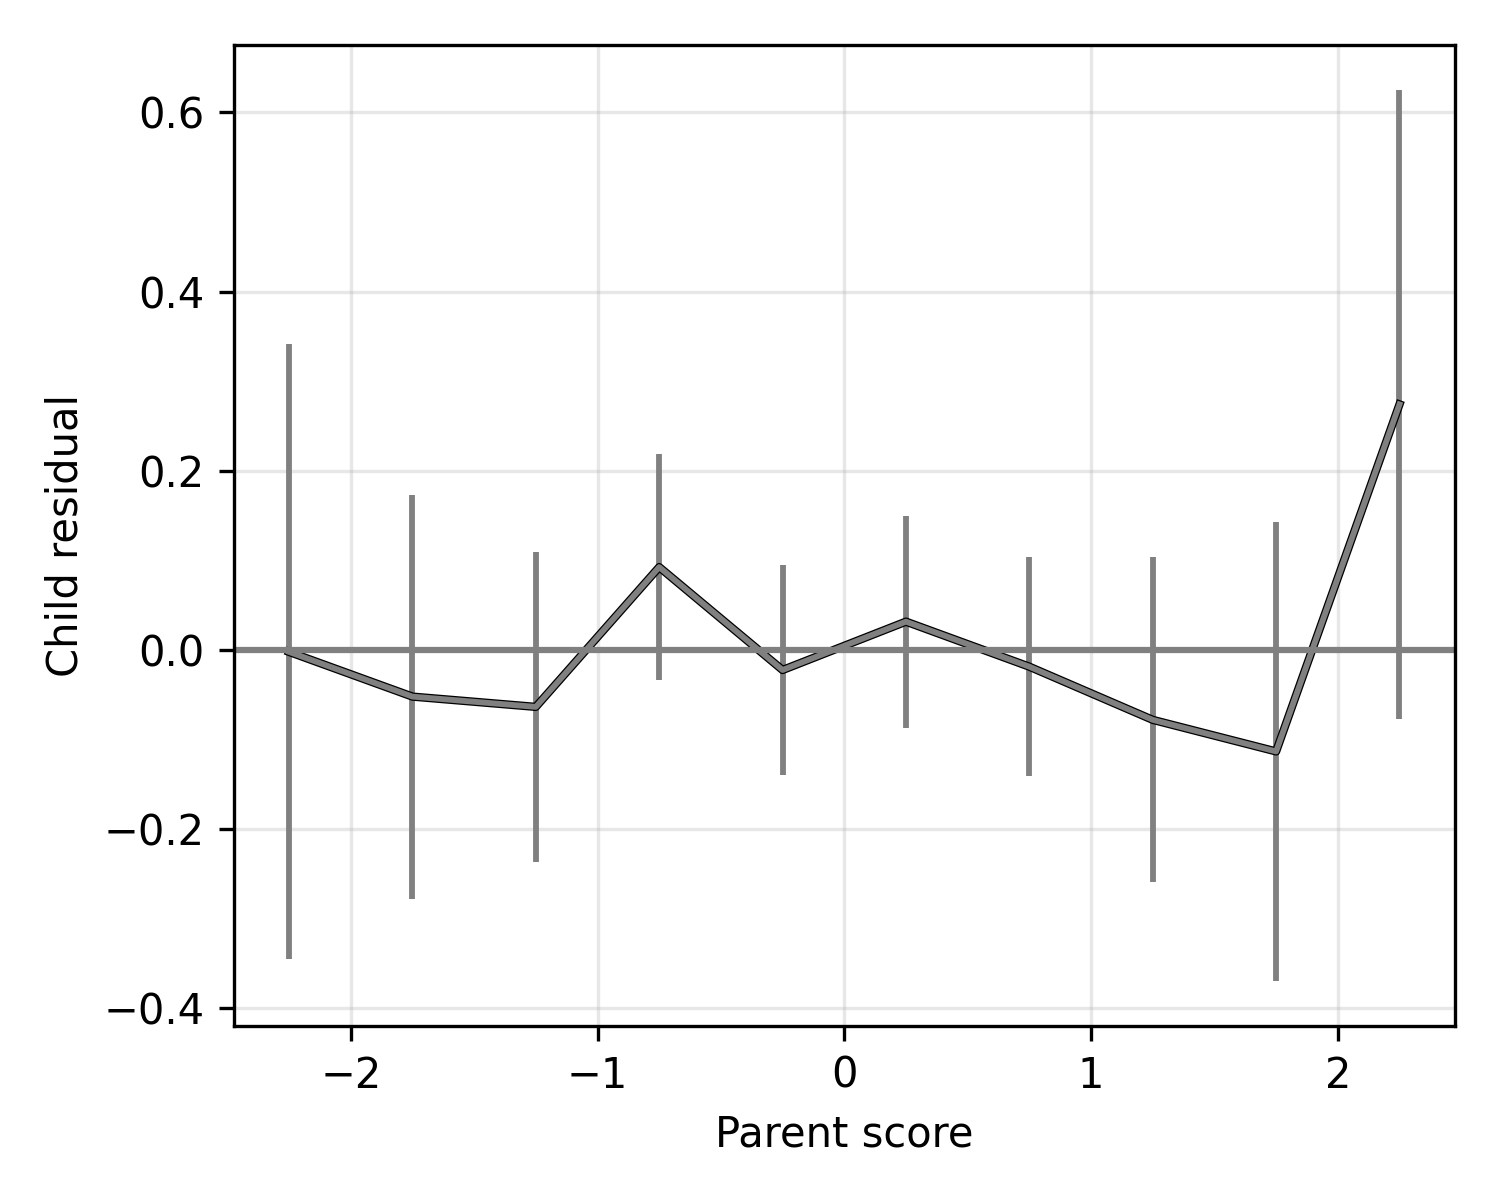
\includegraphics[width=3in]{figures/pearson-lee-mother-daughter-residuals_by_parent.png}
\centering
\caption{Mean values of the residuals by parent score, shown with normal 95\% confidence intervals.}
\label{fig:pearson_residuals_by_score}
\end{figure}

The normality of the daughter generation was also confirmed by Q-Q plot, as well as skewness, kurtosis tests, and D’Agostino and Pearson's test. In summary, we have confirmed from the Pearson female data both the initial condition and the one-step downward transition, and thus the entire model -- as long as there is stable population variance as described earlier. 

Though not shown here, the same statistical tests were applied to the son-father data ($n$ = 1078). All tests passed except the the kurtosis and D'Agostino and Person's test for normality of the residuals and son generation (the skewness tests passed). The failures occurred because of deviations from normality in the edges (more than two standard deviations from the mean) as apparent from the Q-Q plots. These deviations were such that the extremely low and high residuals or scores in the sons generation were lower and higher, respectively, than expected under a normal distribution. 

\subsubsection*{Observed coefficients and population variance dynamics}

The Pearson female data had the estimates $r$ = 0.54 and $r_s$ = 0.96, which nearly produce stable population variance (SD ratio of 1.10). The female data failed the F-test for equality of variances between the mother and daughter generation ($p < 0.001$). The Pearson male data had the estimates $r$ = 0.51 and $r_s$ = 0.89, which nearly produce stable population variance (SD ratio of 1.03). The male data passed the F-test for equality of variances between the father and son generation ($p$ = 0.20). 


Overall, stable population variance seems \emph{a priori} to be a reasonable condition for human stature, though has mixed confirmation in actual data. One possible explanation for why the variance has sometimes been observed to be moderately larger in the child generation is that the children were relatively young adults, and so their heights may have continued to regress towards the mean after the study. Then, their eventual adult heights would have a more similar variance to the heights of their much older parents. This explanation is plausible because, in the Swedish data, all the adult children had their heights measured at around age eighteen \cite{karlberg}. Similarly, in the Pearson data, the adult children had their heights measured when they were eighteen years of age or older \cite{pearson}. 




% MOBILITY AND INFORMATION-LOSS
\section{Mobility and information-loss}

We would like to find some way to quantify the degree of \emph{mobility} in the score of a descendant, given the score of its ancestor. This would also correspond to the \emph{loss of information} about the descendant's score, given its ancestor's score, or vice versa.

\subsection{Mobility as the rate of convergence to the marginal distribution}
For the conditional descendant distribution, faster convergence means that the conditional distribution of the descendant's score quickly becomes indistinguishable from the marginal population distribution of its generation. Information that might precisely predict the descendant's score is \emph{lost} over the intervening generation(s). Faster convergence also means greater mobility, in that -- within few generations -- the descendant's distribution \emph{moves towards} the population distribution (both in expectation and variance). 

For the conditional ancestor distribution, faster convergence means that a descendant's score provides less information about its ancestor's score. 

\subsection{Proposed measure}
We have previously shown that convergence of the conditional distribution to the marginal distribution (both upward and downward) occurs faster with smaller $r$ and larger $r_s$ - and occurs slower for larger $r$ and smaller $r_s$. Accordingly, a simple measure of mobility and information-loss would be proportional to $r$ and inversely proportional to $r_s$. 

Therefore, the simplest way to quantify the mobility and information-loss that occurs between generations is with the following term:

\begin{description}
\item [Definition] Let $m$ be a measure of mobility or equivalently, a measure of information-loss for the Markov process with parameters $r$ and $r_s$:
$$m = \frac{r_s}{r}$$
\end{description}

In general, a value of $m$ is not unique to any given Markov process, because infinitely many values for $r$ and $r_s$ can have the same ratio. Although it is not investigated in detail here, different Markov processes with the same $m$ may turn out to have varied rates of convergence, upwards or downwards, or for expectation or variance. Nonetheless, for stable population variance (the stationary distribution), every possible Markov process has a unique $m$. 


\subsection{Mobility under limiting cases}

We can show with some limiting cases for $r$ and $r_s$ that the desired effects in mobility and information-loss occur, consistent with the proposed measure of mobility. 

\subsubsection*{Small regression coefficient}
Firstly, we consider the limiting case: $r \rightarrow 0$, causing $m \rightarrow \infty$. Then, for small $n$, we have:
$$X_{i+n}|X_i \rightarrow \mathcal{N}(0, \sigma_{i+n}^2)$$
In very few generations, there is nearly a complete loss in information about a descendant's score and there is maximum mobility. 

Likewise, there is also a nearly instantaneous complete loss of information about an ancestor's score, given its descendant's score:
$$X_{i-n}|X_i \rightarrow \mathcal{N}(0, \sigma_{i-n}^2)$$


\subsubsection*{Large residual coefficient}
Next, we consider the limiting case: $r_s \rightarrow \infty$, causing $m \rightarrow \infty$. Then, for small $n$, we have:
$$X_{i+n}|X_i \rightarrow \mathcal{N}(r^nX_i, \infty)$$
Note that the conditional variance rapidly the marginal variance, which goes to infinity:
$$ \tilde{\sigma}_{i+n}^2 \approx \sigma_{i+n}^2 \rightarrow \infty$$
Due to the extremely large variance of the marginal disribution, there is - almost instantly - a nearly complete loss in information about the descendant's score. There is also maximum mobility, as all conditional expectations would have z-scores of approximately zero. 

Likewise, there is also a complete loss in information about the ancestor's score, which converges to the marginal distribution:
$$X_{i-n}|X_i \rightarrow \mathcal{N}(0, \sigma_{i-n}^2)$$


\subsubsection*{Small residual coefficient}
Lastly, we consider the limiting case: $r_s \rightarrow 0$. Because of the degenerate lower bound on $r_s$, shown in Figure \ref{fig:possible_r_rs}, there are two ways for the residual coefficient to approach zero, either the regression coefficient approaches its lower bound of zero or its upper bound of one.

In the first case: $r \rightarrow 0$, it is straightforward to show form the degenerate bound that $r$ must shrink to zero faster than $r_s$ shrinks to zero, such that, if $r$ is made as close as possible to the degenerate bound ($r$ is as great as it possibly can be), we get:
$$r_s^2 \approx r$$
Then, our measure of mobility and information-loss still goes to infinity:
$$m \approx \frac{1}{r_s} \rightarrow \infty$$
Indeed, there is rapid downward convergence to the marginal distribution. For small $n$, we have:
$$X_{i+n}|X_i \rightarrow \mathcal{N}(0, \sigma_{i+n}^2)$$
Likewise, there is also a complete loss in information about the ancestor's score, due to the extremely large population variance and an upper limit on the conditional expectation, such that $\tilde{\mu}_{i-n} < X_i$:
$$X_{i-n}|X_i \rightarrow \mathcal{N}((\frac{r}{r^2+r_s^2})^n X_i, \infty)$$
$$\tilde{\sigma}_{i-n}^2 \approx \sigma_{i-n}^2 \rightarrow \infty$$


In the second case: $r \rightarrow 1$, we get the smallest amount of mobility and information-loss. That is, $m \rightarrow 0$. For small $n$, we have:
$$X_{i+n}|X_i \rightarrow \mathcal{N}(X_i, 0)$$
$$X_{i-n}|X_i \rightarrow \mathcal{N}(X_i, 0)$$
Because we also have $r^2 + r_s^2 \rightarrow 1$, the second case is consistent with stable population variance and the stationary distribution.
$\sigma_{i-n}^2 \approx \sigma_{i-n}^2 \approx 1$
In other words, there is nearly no mobility whatsoever between generations, and very little information is lost about a descendant's or an ancestor's score between generations. That is, an ancestor's score gives an almost perfect prediction of its descendant's score, and vice versa.




%% PROBABILITY KERNELS %%
\section{Probability kernels}

\subsection{State to set, and set to set probabilities}
Let $D$ be a subset of the state space: 
%
$$D \subseteq \mathbb{R}$$

\begin{description}
\item [Definition] The probability kernel $P_n(D, x_i)$ is the $n$-step probability of reaching the set $D$ in the descendant population from the state $x_i$ in the ancestor population.
$$P_n(D, x_i) = \int_{x_{i+n}\in D}^{} f(x_{i+n}|x_i)f(x_i) \, dx_{i+n}$$
\end{description}

Where $f(x_{i+n}|x_i)$ is the conditional probability density function (pdf) of $X_{i+n}|X_i \sim \mathcal{N}( \tilde{\mu}_{i+n}, \tilde{\sigma}_{i+n})$, and $f(x_i)$ is the pdf of $X_i \sim \mathcal{N}(0, \sigma_i^2)$.
The expression can be simplified to the following, as long as $D$ is the uninterrupted set $(D_{min}, D_{max})$:

$$P_n(D, x_i) = f(x_i)[\, \Phi(\frac{D_{max}- \tilde{\mu}_{i+n}}{\tilde{\sigma}_{i+n}}) - \Phi(\frac{D_{min}- \tilde{\mu}_{i+n}}{\tilde{\sigma}_{i+n}}) \, ]$$

Where $\Phi$ is the cumulative density function (cdf) of the standard normal distribution. 

Let $A$ also be a subset of the state space:
%
$$A \subseteq \mathbb{R}$$

\begin{description}
\item [Definition] A similar probability kernel $P_n(D, A)$ is the $n$-step probability of reaching the set $D$ in the descendant population from the set $A$ in the ancestor population. 
$$P_n(D, A) = \int_{x_i\in A}^{} P_n(D, x_i) \, dx_i$$
\end{description}

The stationary distribution arises from stable population variance, in which we have $f(x_1|x_2)f(x_2) = f(x_2|x_1)f(x_1) = f(x_1, x_2)$ for any $x_1$, $x_2$, where $f(\cdot|\cdot)$ has the form $f(x_{i+n}|x_i)$ (describing the conditional descendant distribution). Therefore, under stable population variance, we have: 
$$P_n(D, A) = P_n(A, D)$$
To show this, we let $d = i+n$ be the notation for the conditional ancestor distribution, then we have $f(x_{i+n}|x_i)f(x_i) = f(x_{d-n}|x_d)f(x_d)$ in all cases (for both stable and unstable population variance). However, under the time-reversibility of stable population variance, we also have $f(x_{d-n}|x_d)f(x_d) = f(x_{i}|x_{i+n})f(x_{i+n})$, where the right hand side is the form of the conditional descendant distribution. Thus we have shown the result. 

It should also be noted that when $x_1$ and $x_2$ are calculated from percentiles, the result is akin to the that of stable population variance, because the values are normalized to the differing variances of the two generations. That is for any two percentiles $p_1$ and $p_2$, we have: 
$$f(F_{i+n}^{-1}(p_1)|F_i^{-1}(p_2))f(F_i^{-1}(p_2)) = f(F_{i+n}^{-1}(p_2)|F_i^{-1}(p_1))f(F_i^{-1}(p_1))$$
Where $f(\cdot|\cdot)$ has the form $f(x_{i+n}|x_i)$ as before, and $F_{\cdot}^{-1}(p)$ is the inverse cumulative density function of generation $i$ or $i+n$. Therefore, when $Q_j$ and $Q_k$ are percentile sets, we have:
$$P_n(Q_j, Q_k) = P_n(Q_k, Q_j)$$ 
Where the notation implies a conversion to real numbers of the form: $P_n(F_{i+n}^{-1}(Q_j), F_i^{-1}(Q_k)$. This results in a persymmetry property described in the section on percentile transition matrices. 


% ATTRIBUTABLE
\subsection{Attributable and destined probabilities}

\begin{description}
\item [Definition] $P_{\alpha , n}(D, A)$ is the probability that a state $X_{i+n}$ in set $D$ is descendant from or is \emph{attributable} to an ancestor state $X_i$ in set $A$.
$$P_{\alpha , n}(D, A) = \frac{P_n(D, A)}{P_n(D, \mathbb{R})}$$
\end{description}

By the law of total probability, $P_n(D, \mathbb{R})$ is the marginal probability that the state $X_{i+n}$ is in the space $D$, this can be obtained by the cumulative density function of a normal distribution by the following definition.

\begin{description}
\item [Definition] For some arbitrary subset of the state space $S \subseteq \mathbb{R}$, $P(S)$ is the marginal probability that the normally distributed rv $X \sim \mathcal{N}(\mu, \sigma^2)$ is in the subset $S$. The last equality holds if $S$ is the uninterrupted set $(S_{min}, S_{max})$.
$$P(S) = \int_{x\in S} f(x) \, dx = \Phi(\frac{S_{max} - \mu}{\sigma}) - \Phi(\frac{S_{min} - \mu}{\sigma})$$
\end{description}

For $P(D)$, its integrand $f(x)$ would be the pdf of $X_{i+n} \sim \mathcal{N}(0, \sigma_{i+n}^2)$. Therefore:
$$P_{\alpha , n}(D, A) = \frac{P_n(D, A)}{P(D)}$$


% DESTINED

\begin{description}
\item [Definition] $P_{\delta , n}(D, A)$ is the probability that a state $X_i$ in set $A$ has a descendant state $X_{i+n}$ that appears in or is \emph{destined} for the set $D$. 
$$P_{\delta , n}(D, A) = \frac{P_n(D, A)}{P_n(\mathbb{R}, A)}$$
\end{description}

It can be shown by the fact that an integral over the entire support of a pdf equals one, that $P_n(\mathbb{R}, A)$ is the marginal probability that the state $X_i$ is in the set $A$, which is given by $P(A)$. Therefore:
%
$$P_{\delta , n}(D, A) = \frac{P_n(D, A)}{P(A)}$$


It should be noted that when attributable and destined probability calculations are generally made on a relative basis, they are not distorted by unstable population variance. Specifically, for the percentile sets $Q_j$ and $Q_k$, the descendant population may have a very large or small variance relative to the ancestor population, especially if $n$ is large, however, this is made immaterial by the standardization involved in calculating from percentiles.

% PERCENTILE TRANSITION MATRICES
\subsection{Percentile transition matrices}

The calculations of attributable and destined probabilities can be defined by percentile sets, as introduced earlier. For example, in $P_{\delta , n}(Q_j, Q_k)$, the percentile set $Q_k$ would be converted to a real number set through $F_i^{-1}(Q_k)$, using the marginal population variance $\sigma_i^2$ of population $i$. 

Percentile transition matrices result from equal-size, continuous percentile sets $Q_1$, $Q_2$, ..., $Q_m$. For example, for $m=5$, we have: $Q_1 = \left(0, 0.2\right]$, $Q_2 = \left(0.2, 0.4\right]$, ..., $Q_m = \left(0.8, 1\right]$. Because, all percentile sets have the same size, e.g., $P(Q_j) = P(Q_k) = 0.2$, the calculations can be equivalently interpreted as attributable and destined probabilities. That is, we have, for all $j$, $k$:
$$P_{\alpha , n}(Q_j, Q_k) = P_{\delta , n}(Q_j, Q_k) = P_{\cdot , n}(Q_j, Q_k)$$

\begin{description}
\item [Definition] The percentile transition matrix is defined as follows for continuous, equal-size percentile sets $Q_1$, $Q_2$, ..., $Q_m$:
 $$
\begin{pmatrix}
P_{\cdot , n}(Q_m, Q_1) &  P_{\cdot , n}(Q_m, Q_2)  & \ldots & P_{\cdot , n}(Q_m, Q_m)\\
P_{\cdot , n}(Q_{m-1}, Q_1)  &  P_{\cdot , n}(Q_{m-1}, Q_2) & \ldots & P_{\cdot , n}(Q_{m-1}, Q_m)\\
\vdots & \vdots & \ddots & \vdots\\
P_{\cdot , n}(Q_1, Q_1)  &   P_{\cdot , n}(Q_1, Q_2)       &\ldots & P_{\cdot , n}(Q_1, Q_m)
\end{pmatrix}
$$
\end{description}
 
Simulated and observed percentile transition matrices are shown in Figures \ref{fig:quintile_pearson}, \ref{fig:quintile_stable}, and \ref{fig:quintile_mobility}, and \ref{fig:quintile_chetty}, with the rows indicated by color, and the sizes proportional to the probabilities. One way to understand these matrices is to consider an entry as a proportion of its column sum (indicating probability or proportion destined) or row sum (indicating probability or proportion attributable). Because the quintiles in the ancestor and descendant generations are the same size, e.g., 20\%, the column sums and row sums must both add to 100\% (with any deviations due to rounding). 

\subsubsection*{Bisymmetry of percentile transition matrices}

Theoretical percentile transition matrices are bisymmetric (symmetric along both diagonals). This can be proved by showing them to be both persymmetric (symmetric along the northeast to southwest diagonal) and symmetric (symmetric along the northwest to southeast diagonal). 

We discussed in the section on set to set probabilities, how $P_n(Q_j, Q_k) = P_n(Q_k, Q_j)$. Therefore, assuming  $P(Q_j) = P(Q_k)$ as before, we also have for percentile transition matrices: 
$$P_{ \cdot, n}(Q_j, Q_k) = P_{\cdot, n}(Q_k, Q_j)$$
An example of the persymmetry property is that the probability relating parents in the bottom quintile to children in the second quintile is the same as that relating parents in the second quintile to children in the bottom quintile.

The symmetry property results from the fact that normal distributions are symmetric, which means that $f(-x_1,-x_2) = f(x_1,x_2)$ (under the conditional descendant distribution). Combining this fact with the earlier one, we get $f(x_1|x_2)f(x_2) = f(-x_2|-x_1)f(-x_1)$, which is equivalent to percentile transition matrices being symmetric. The symmetry property can be written as follows:
$$P_{ \cdot, n}(Q_j, Q_k) = P_{\cdot, n}(Q_{m-k+1}, Q_{m-j+1})$$
An example of the symmetry property is that the probability relating parents in the bottom quintile to children in the fourth quintile is the same as that relating parents in the second quintile to children in the top quintile. Because of the symmetry property, the simulated matrices in Figures \ref{fig:quintile_pearson}, \ref{fig:quintile_stable}, and \ref{fig:quintile_mobility}, can equivalently be re-written with the x-axis as \emph{Descendant's} or \emph{Child's Quintile}, and the y-axis as \emph{Cumulative Probability of Parent's} or \emph{Ancestor's Quintile}. 

One result of bisymmetry is that the number of unique entries in a theoretical percentile transition matrix is far fewer than the number of entries in the matrix. The number of unique entries in an $m \times m$ bisymmetric matrix has an additive analogy of $m!!$ unique, or independent, entries. This can be shown by a simple geometric argument: filling in the entries by row, in which for every new iteration, the outer two entries are non-unique. That is, the number of unique entries in an $m \times m$ percentile transition matrix is $m + (m-2) + (m-4) + ... + 4 + 2$ for even $m$, and $m + (m-2) + (m-4) + ... + 3 + 1$ for odd $m$. This is an arithmetic series, and the sum of an arithmetic series with $n$ terms is always $S_n = n(a_1 + a_n) /2$, where $a_1$ is the smallest term and $a_n$ is the largest term (the gap between successive terms is irrelevant). Then it is straightforward to show that the number of unique entries is $m(m+2)/4$ for even $m$, and for $(m+1)^2/4$ for odd $m$. Therefore, the simulated quintile-transition matrices shown in this paper, for which $m = 5$, have 25 total entries, but only 9 unique entries.



\subsection{Visualizations of percentile transition matrices}

\subsubsection*{Comparison to Pearson data}

The observed percentile transition matrices of the Pearson mother-daughter and father-son data are shown along with a simulation from the estimated parameters in Figure \ref{fig:quintile_pearson}. A reasonable similarity is observed between the simulated and observed matrices. It should be noted that for the Pearson data, there was a relatively small number of observations for each entry of the quintile-quintile matrices (average of 49, minimum of 10, and maximum of 149). This may explain some of the disagreement between the male and female matrices, and potentially also the deviations from the simulated matrix. 

The rightmost column in Figure \ref{fig:quintile_pearson} shows that for stature, a parent in the top quintile has about a 43\% chance of having a child also in (destined for) the top quintile, a 25\% chance of having a child (of the same sex) in the fourth quintile, an 18\% chance of having a child in the middle quintile, and so on. Equivalently, these numbers can be interpreted as follows: about 43\% of the children in the top quintile is attributable to parents (of the same sex) also in the top quintile, 25\% of the children in the fourth quintile are attributable to parents in the top quintile, 18\% of the children in the middle quintile is attributable to parents in the top quintile, and so on. 

\begin{figure}[H]
\centering
\advance\leftskip-0.4in
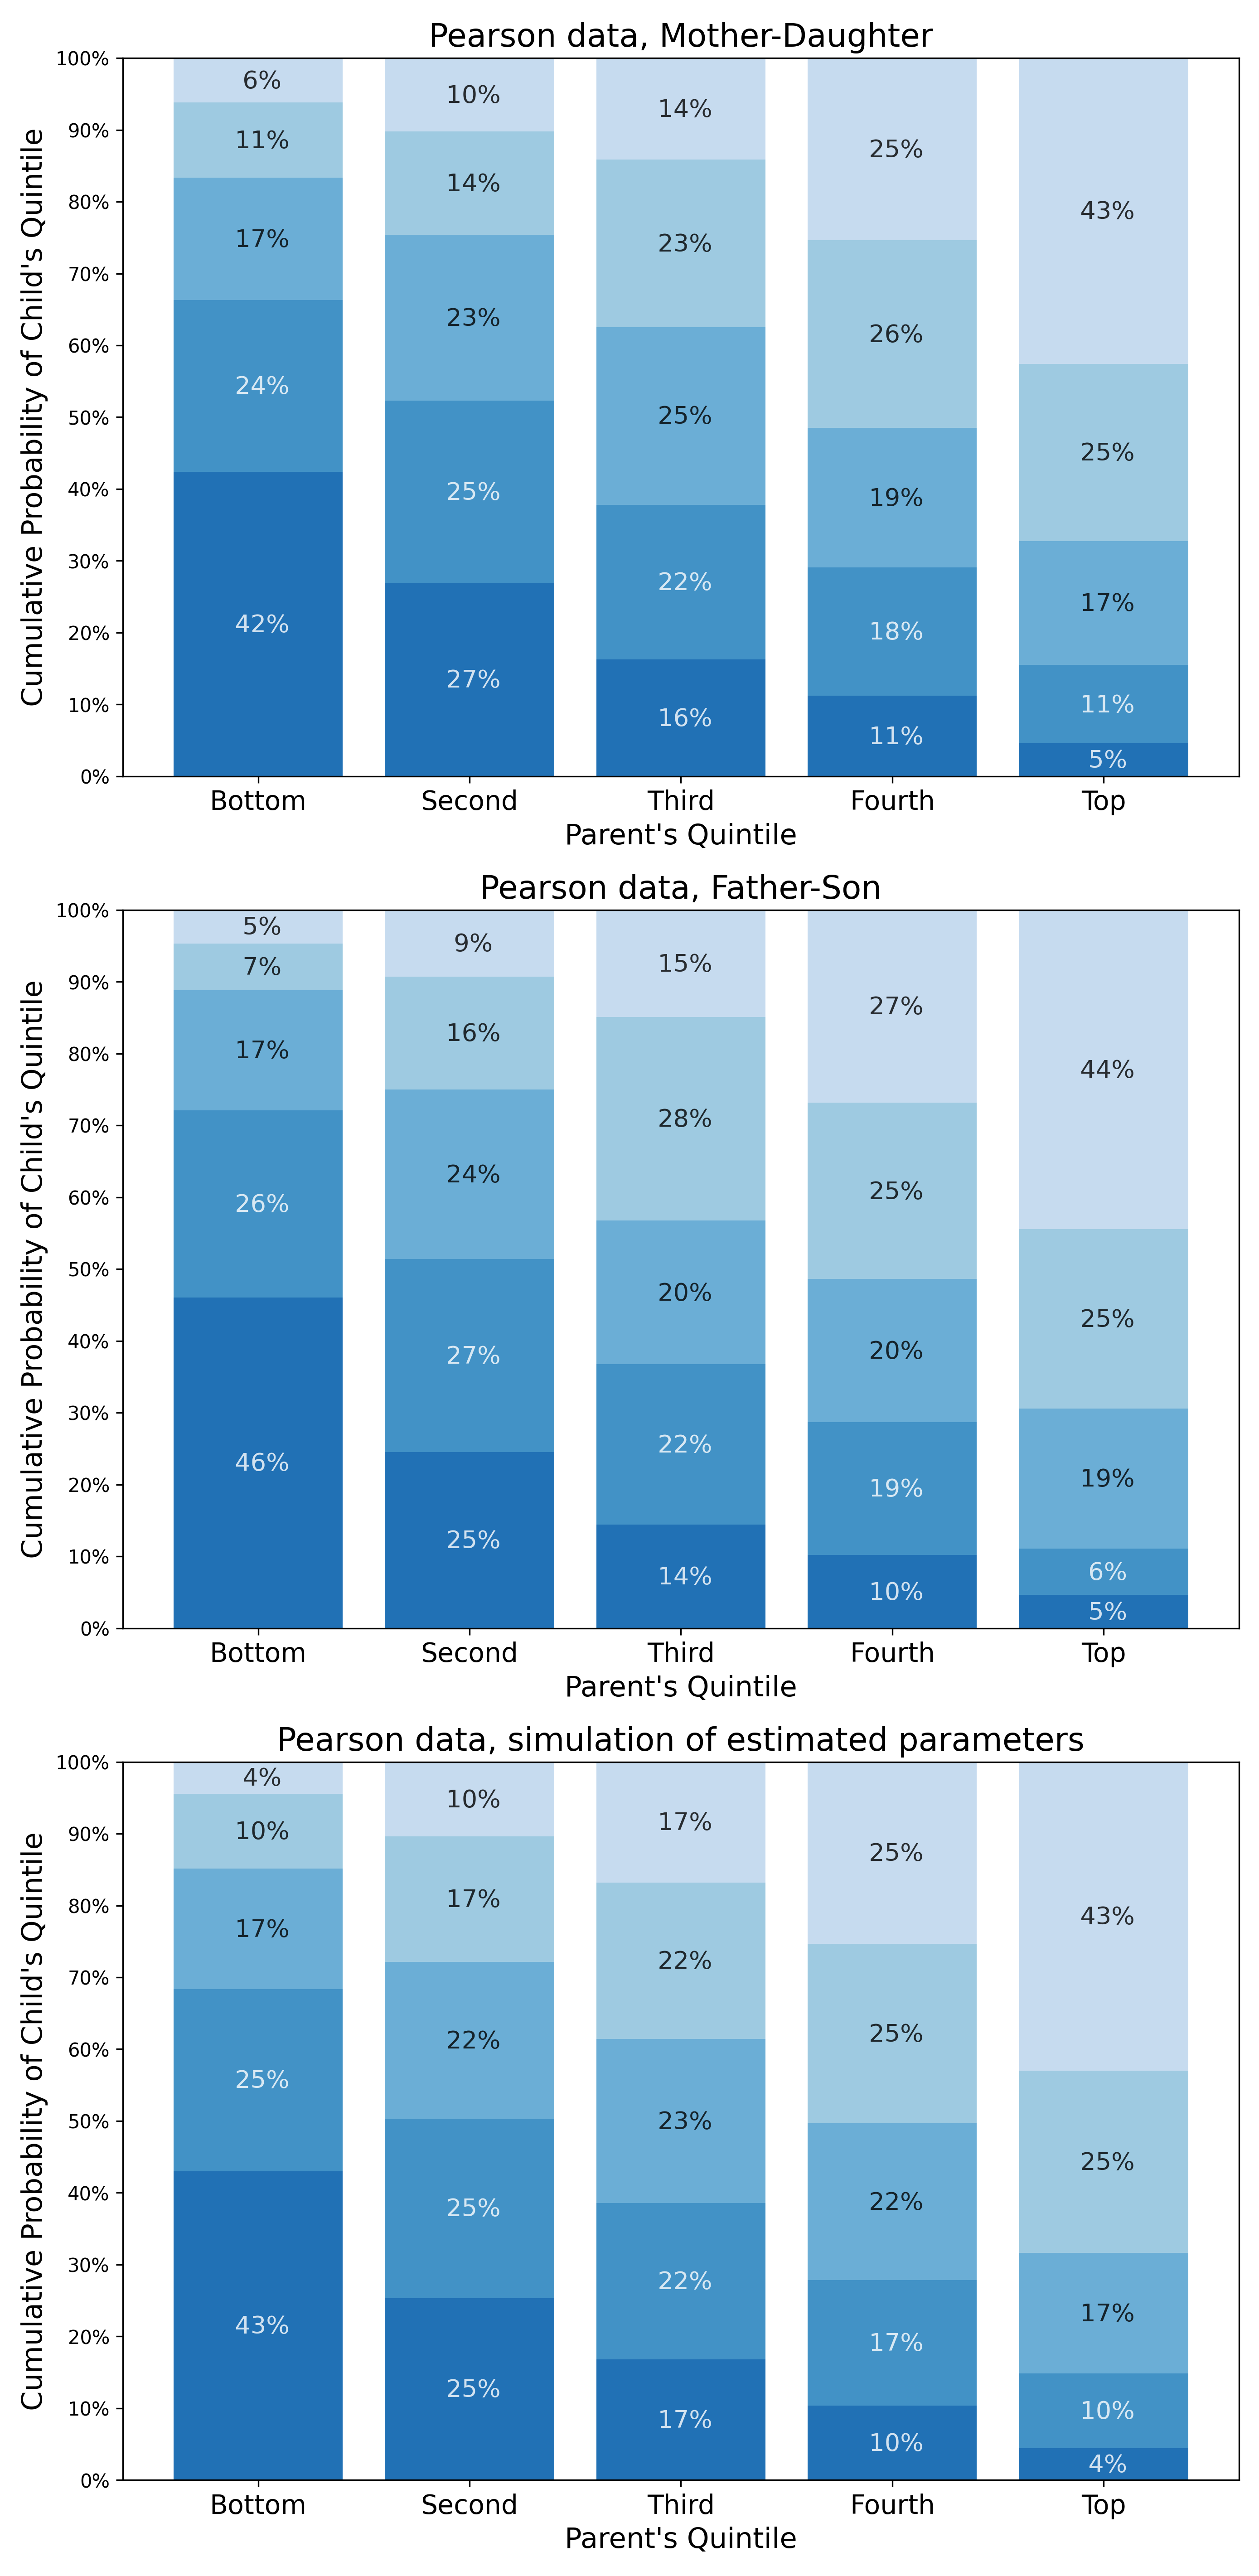
\includegraphics[width=3.5in]{figures/quintile-pearson.png} 
\caption{Observed and simulated quintile transition matrices from the Pearson data, with estimated parameters $r = 0.54$, $r_s = 0.96$ for female and $r = 0.51$, $r_s = 0.89$ for male \cite{pearson}. These parameters result in identical simulated matrices (to the first decimal place), therefore only one is shown.}
\label{fig:quintile_pearson}
\end{figure}

\subsubsection*{Multigenerational regression towards the mean}
Between the Pearson and Swedish data on stature, the estimates for $r$ were about 0.5, with approximately stable population variance. Using $r = 0.5$ and stable population variance ($r_s \approx 0.866$), percentile transition matrices can be simulated, showing the regression towards the mean that takes place over multiple generations. Quintile transition matrices of this form are shown in Figure \ref{fig:quintile_stable}. The exponential convergence to the descendant distribution can be seen in the asymptotic approach of the probabilities towards uniform 20\%, with slowing rates of convergence as the generation-gap widens. 

\begin{figure}[H]
\centering
\advance\leftskip-0.6in
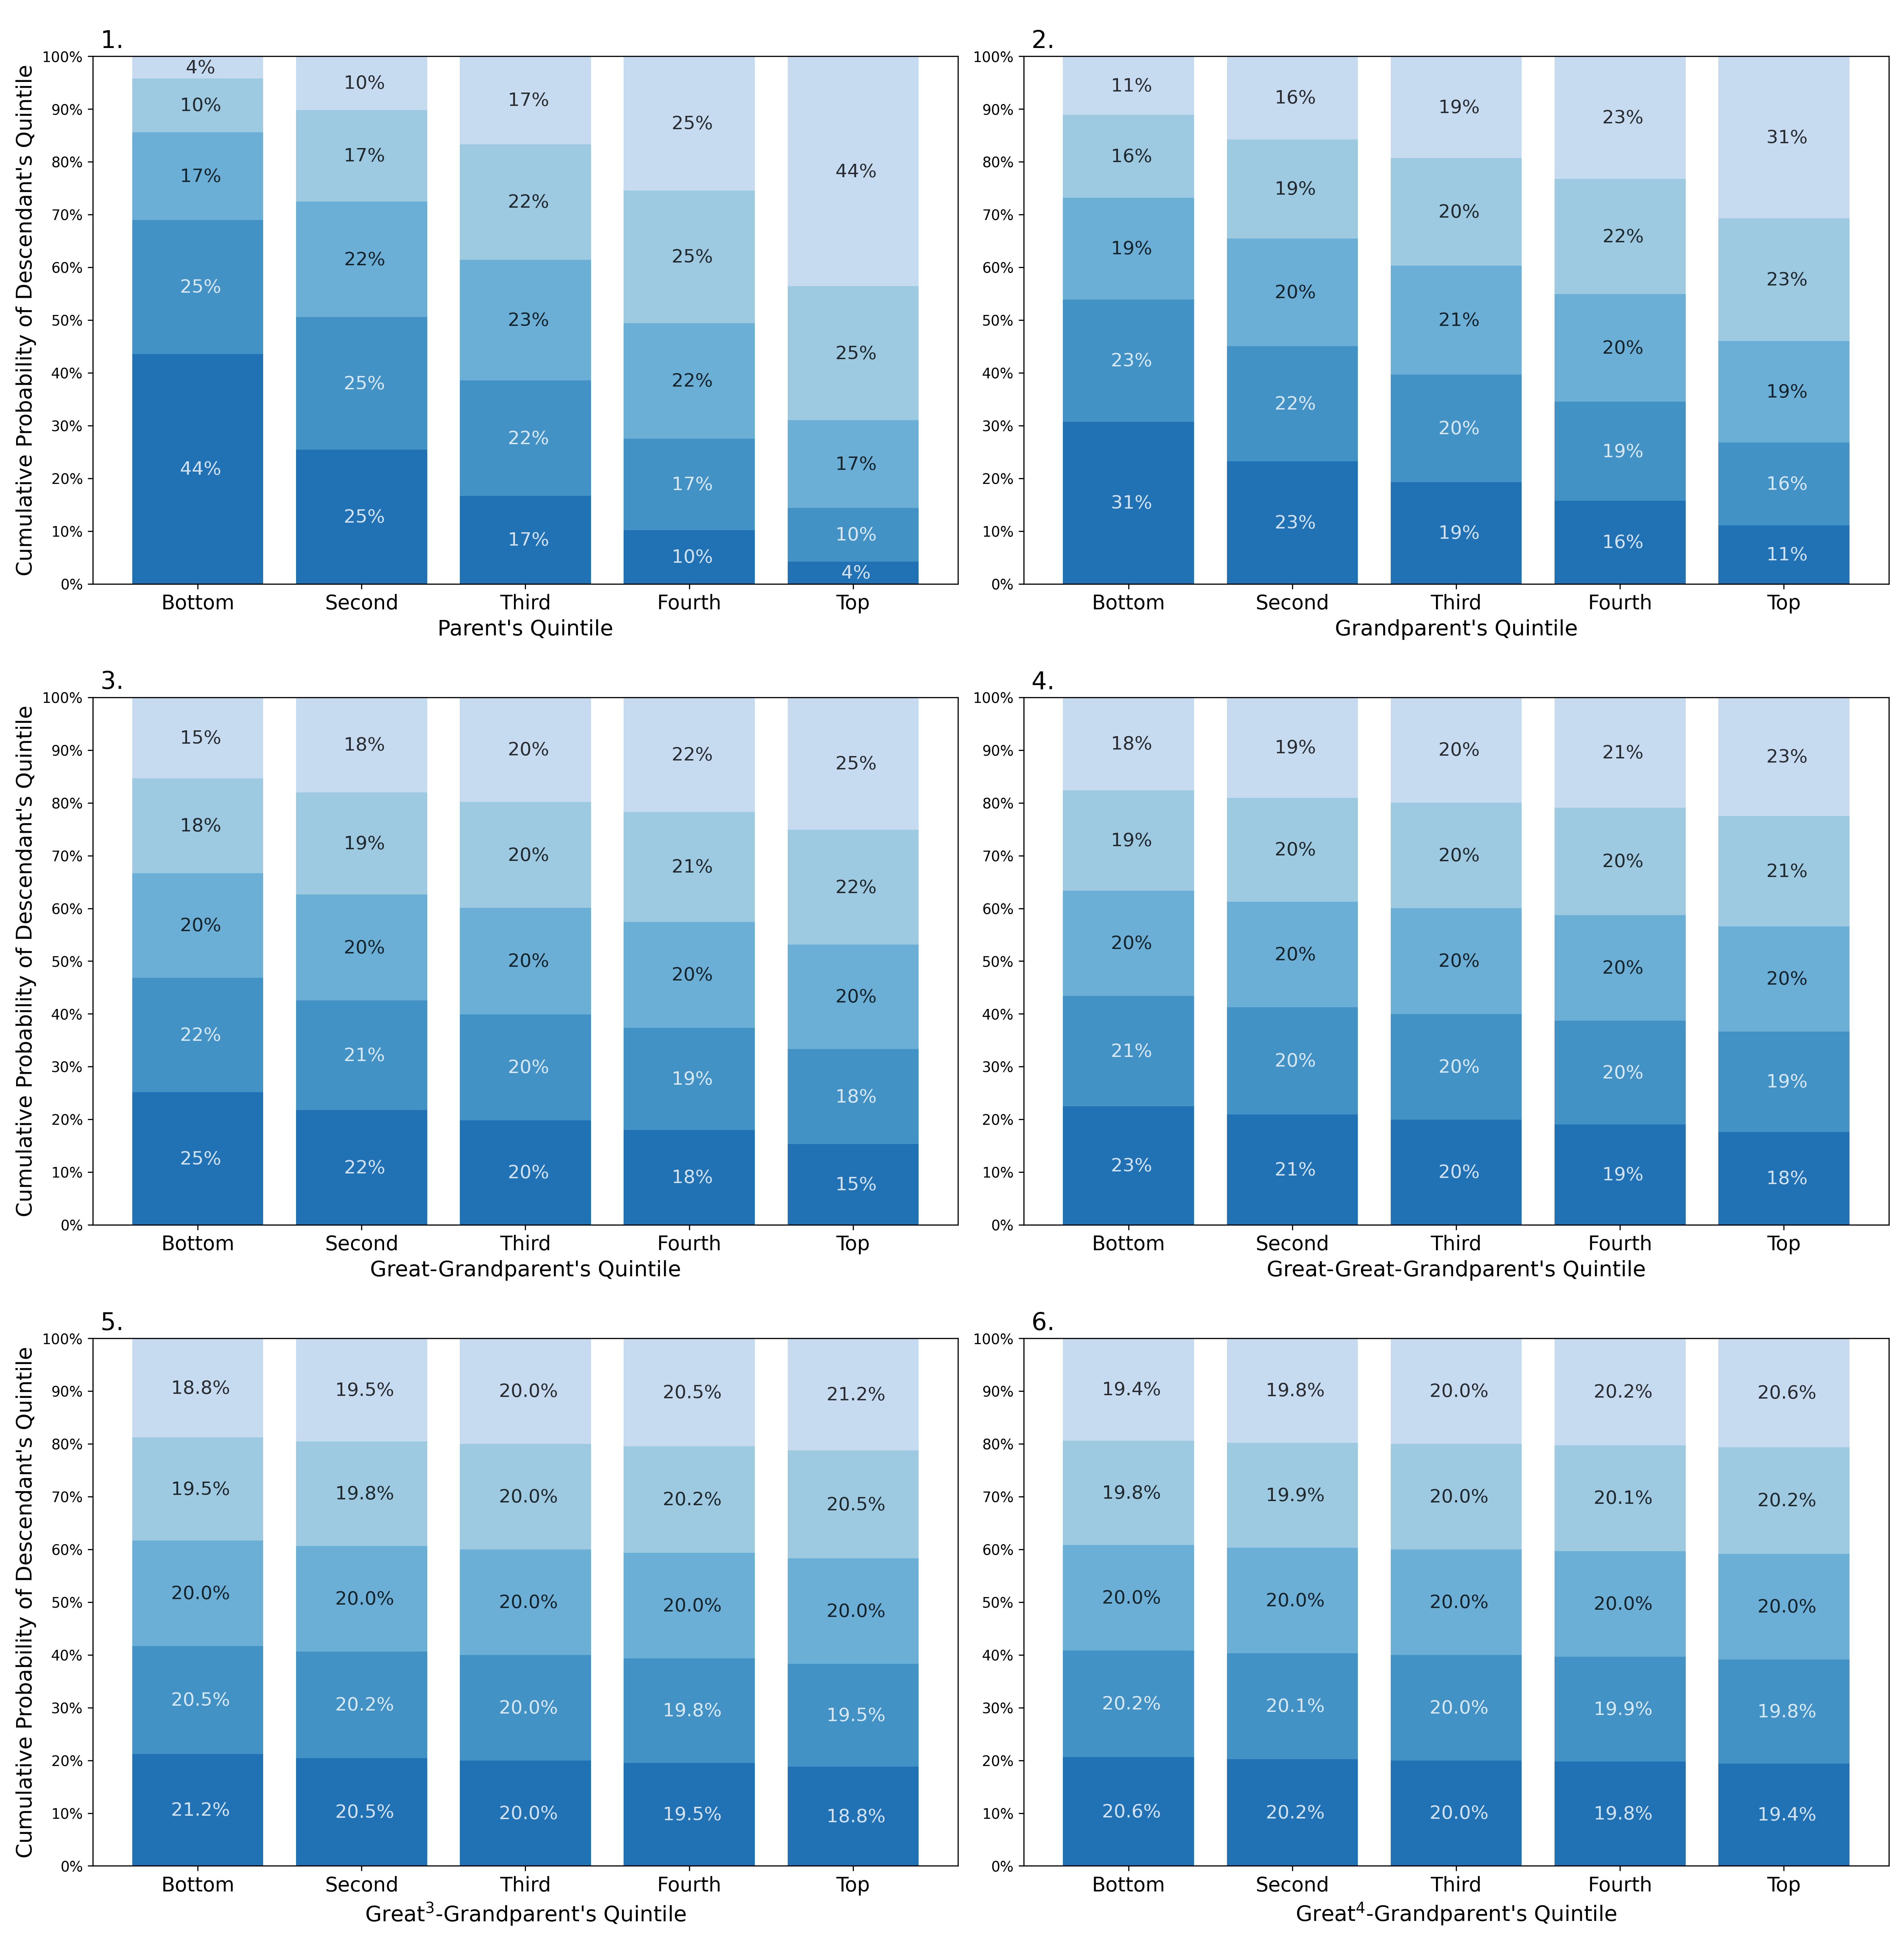
\includegraphics[width=6.5in]{figures/quintile-r=0.5-stable.png} 
\caption{Quintile transition matrices over generation-gaps $n$ from 1 through 6, with stable population variance at $r = 0.5$ ($r_s \approx 0.866$).}
\label{fig:quintile_stable}
\end{figure}

\subsubsection*{Visualization of the mobility measure}
The effect of the mobility measure $m$ introduced earlier, where $m = \frac{r_s}{r}$, can be visualized in percentile transition matrices with varying $m$. Quintile transition matrices of this form are shown in Figure \ref{fig:quintile_mobility} under stable population variance, for which $m$ uniquely describes the distribution.


\begin{figure}[H]
\centering
\advance\leftskip-0.6in
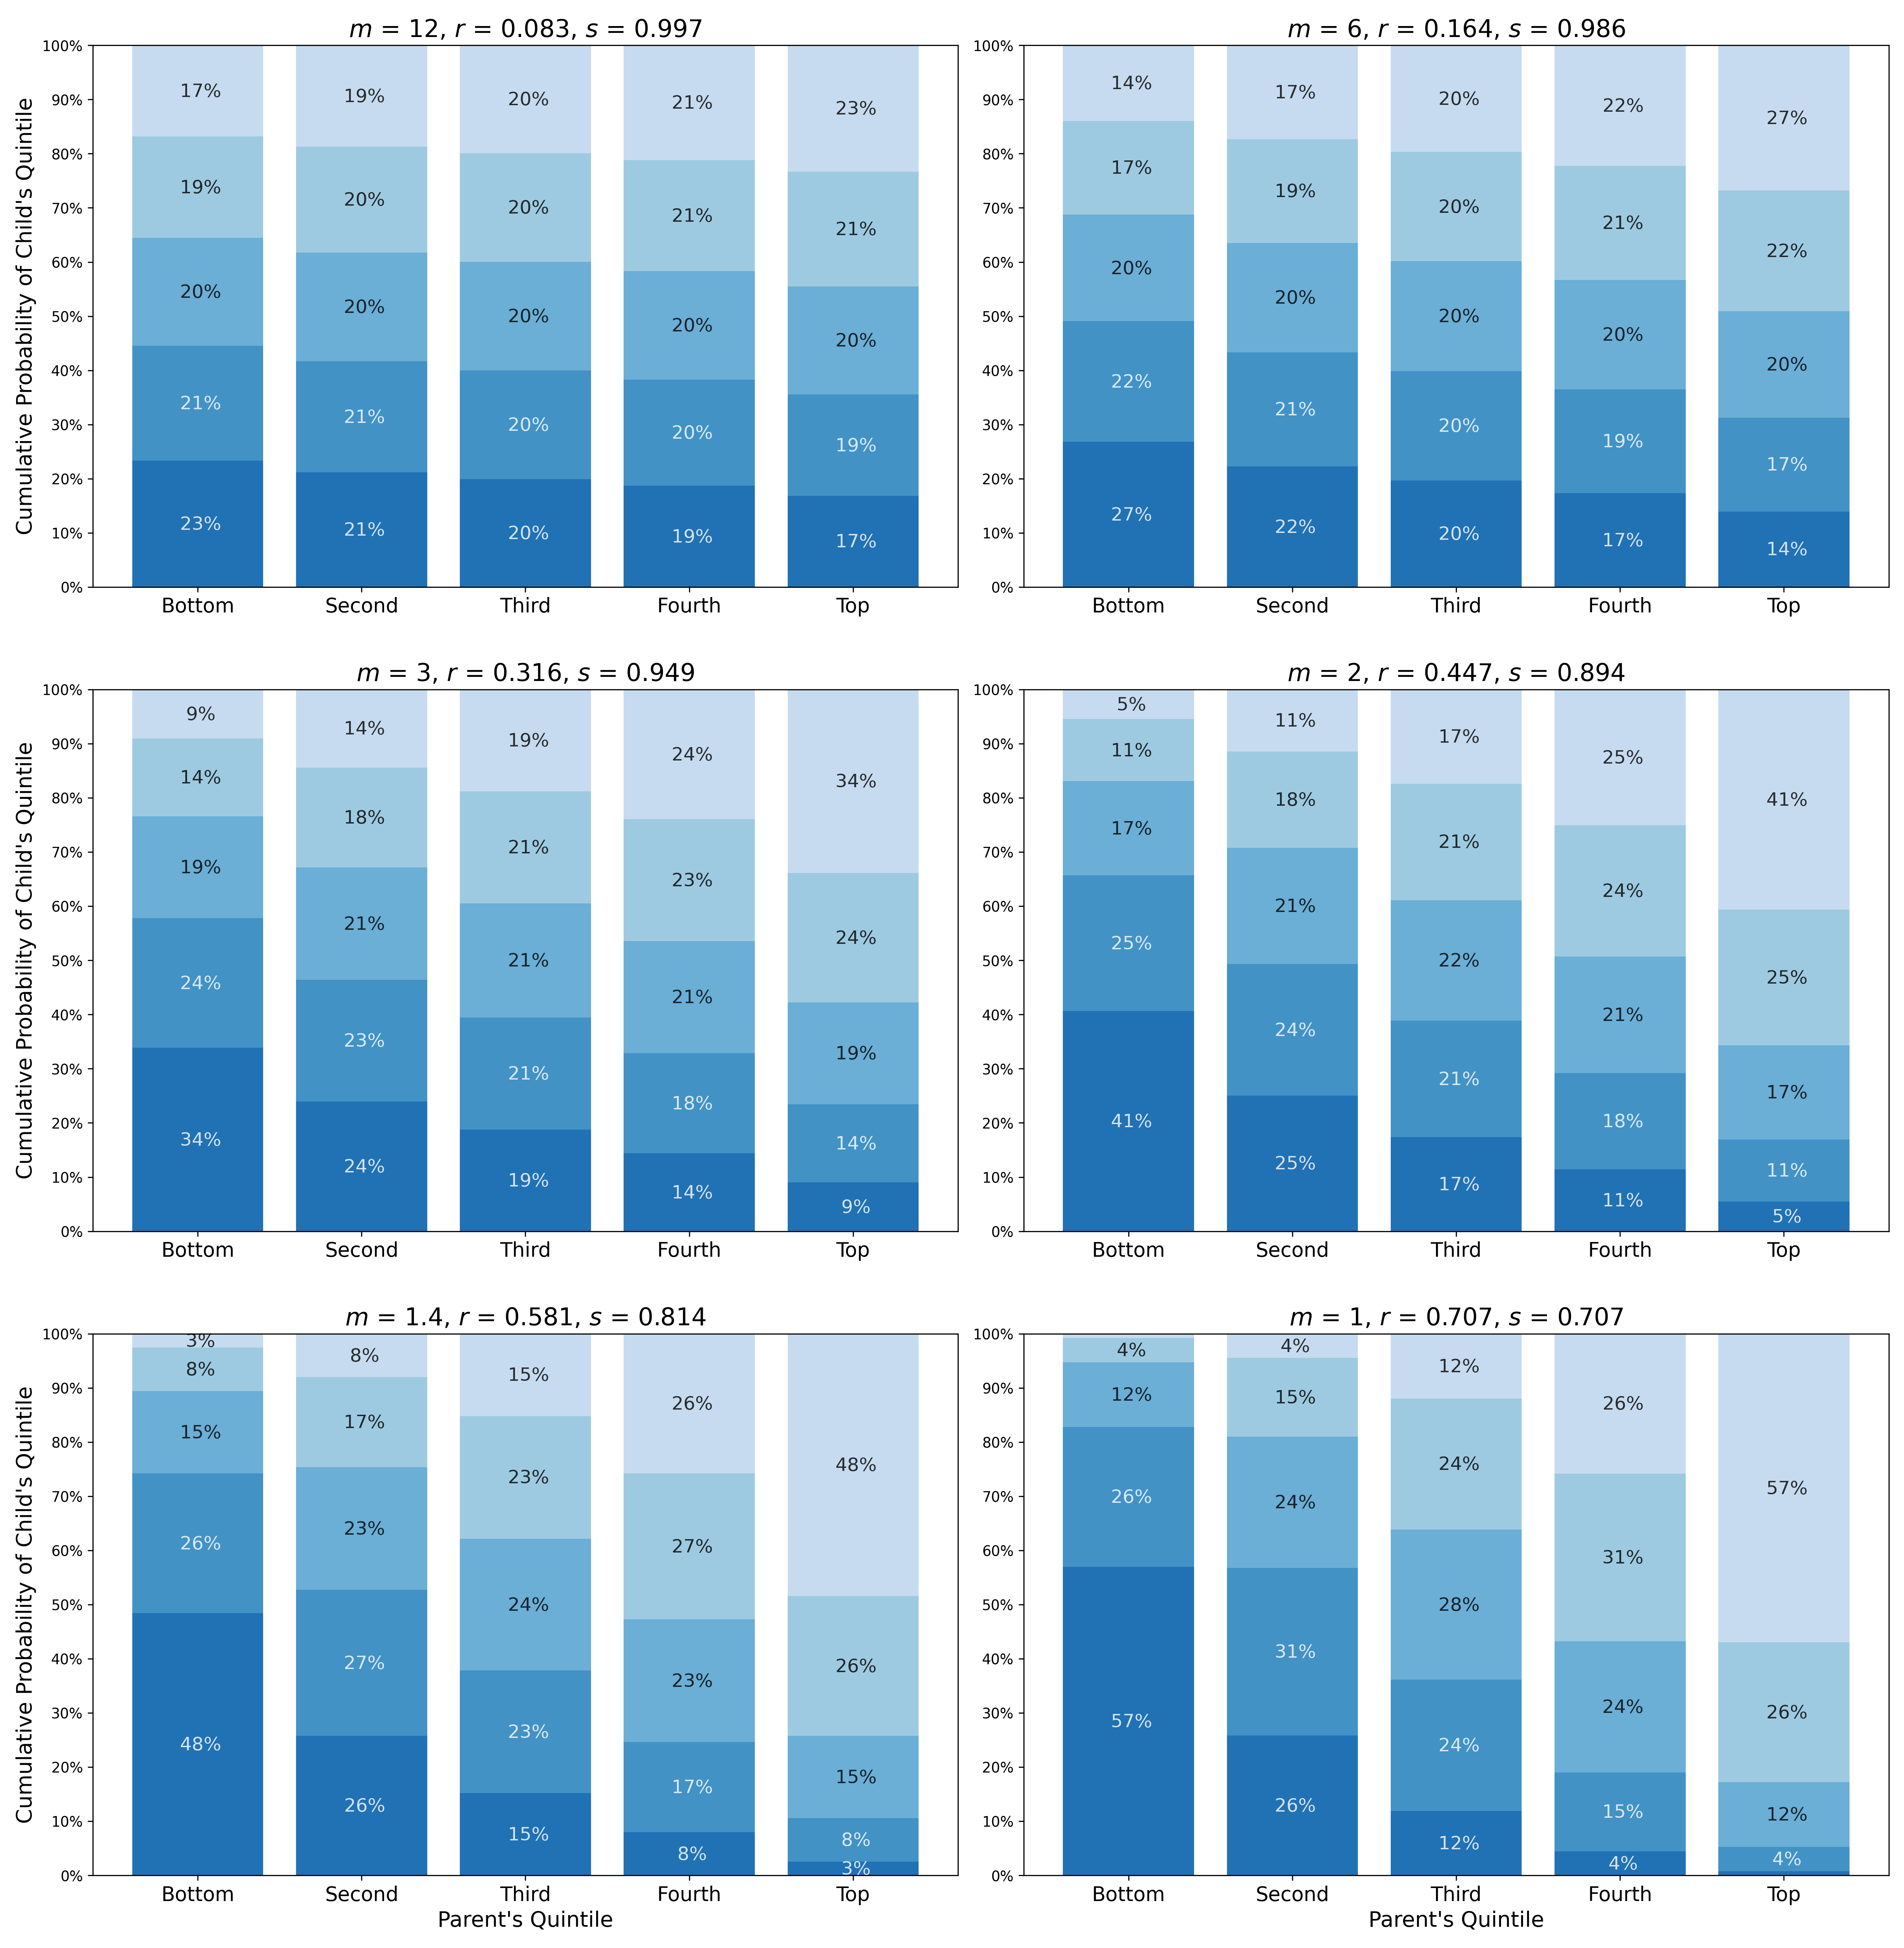
\includegraphics[width=6.5in]{figures/quintile-mobility.png} 
\caption{Parent-to-child quintile transition matrices, over decreasing levels of mobility, with stable population variance.}
\label{fig:quintile_mobility}
\end{figure}


\subsubsection*{Comparison to US family income mobility}

A quintile transition matrix relating the family incomes of 9,867,736 US children born between 1980-82 and their parents has been calculated from tax-data, shown in Figure \ref{fig:quintile_chetty} \cite{chetty}. This transition matrix is crucially different than the other ones shown in this paper because it relates measures of the \emph{families} of children and their parents, rather than relating measures of an individual child to one of its parents (of the same sex). Nonetheless, reasons for similarity can be explained by the fact that the distribution of income can be approximated by a log-normal distribution \cite{battistin, neal}. Percentiles (and their corresponding transition matrices) are unaffected by this transformation because taking the logarithm is a monotonic function. Then, if the relation between the (log) income of parents and their children can be roughly approximated by a normal linear model, the Markov process model described in this paper could reasonably be applied.

If there is a positive correlation between the income of a child and the income of his or her parent, then the correspondence should be greater (and mobility lower) when using the parent's \emph{family} income (rather than only one of the parent's income), because measuring family income combines the incomes of all parents. On the other hand, if there is a correlation of less than one between a child's income and the incomes of his or her parents, the correspondence should be lower (and mobility greater), when using the child's \emph{family} income (rather than the child's individual income). 

Whether these two opposing effects on mobility cancel out precisely depends on whether the correlation between individual and family income is the same for both the child and parent generations, or whether such correlations vary between income quintile. These are both unknown, thus the caveat must be made that the transition matrix in Figure \ref{fig:quintile_chetty} cannot be equivalently compared to the other transition matrices shown in this paper. Nonetheless, it can be generally remarked that there is a greater degree of observed mobility in family income (Figure \ref{fig:quintile_chetty}) than in stature (Figure \ref{fig:quintile_pearson}). More precisely, mobility measure for income appears to be best approximated by $m \approx 3$, for which there is a corresponding quintile transition matrix in Figure \ref{fig:quintile_mobility}. This can be compared with the mobility of height (which has a much larger genetic determinant) of about $m \approx$ 1.7-1.8, obtained from the estimates of the regression and residual coefficients.

\begin{figure}[H]
\centering
\advance\leftskip-0.4in
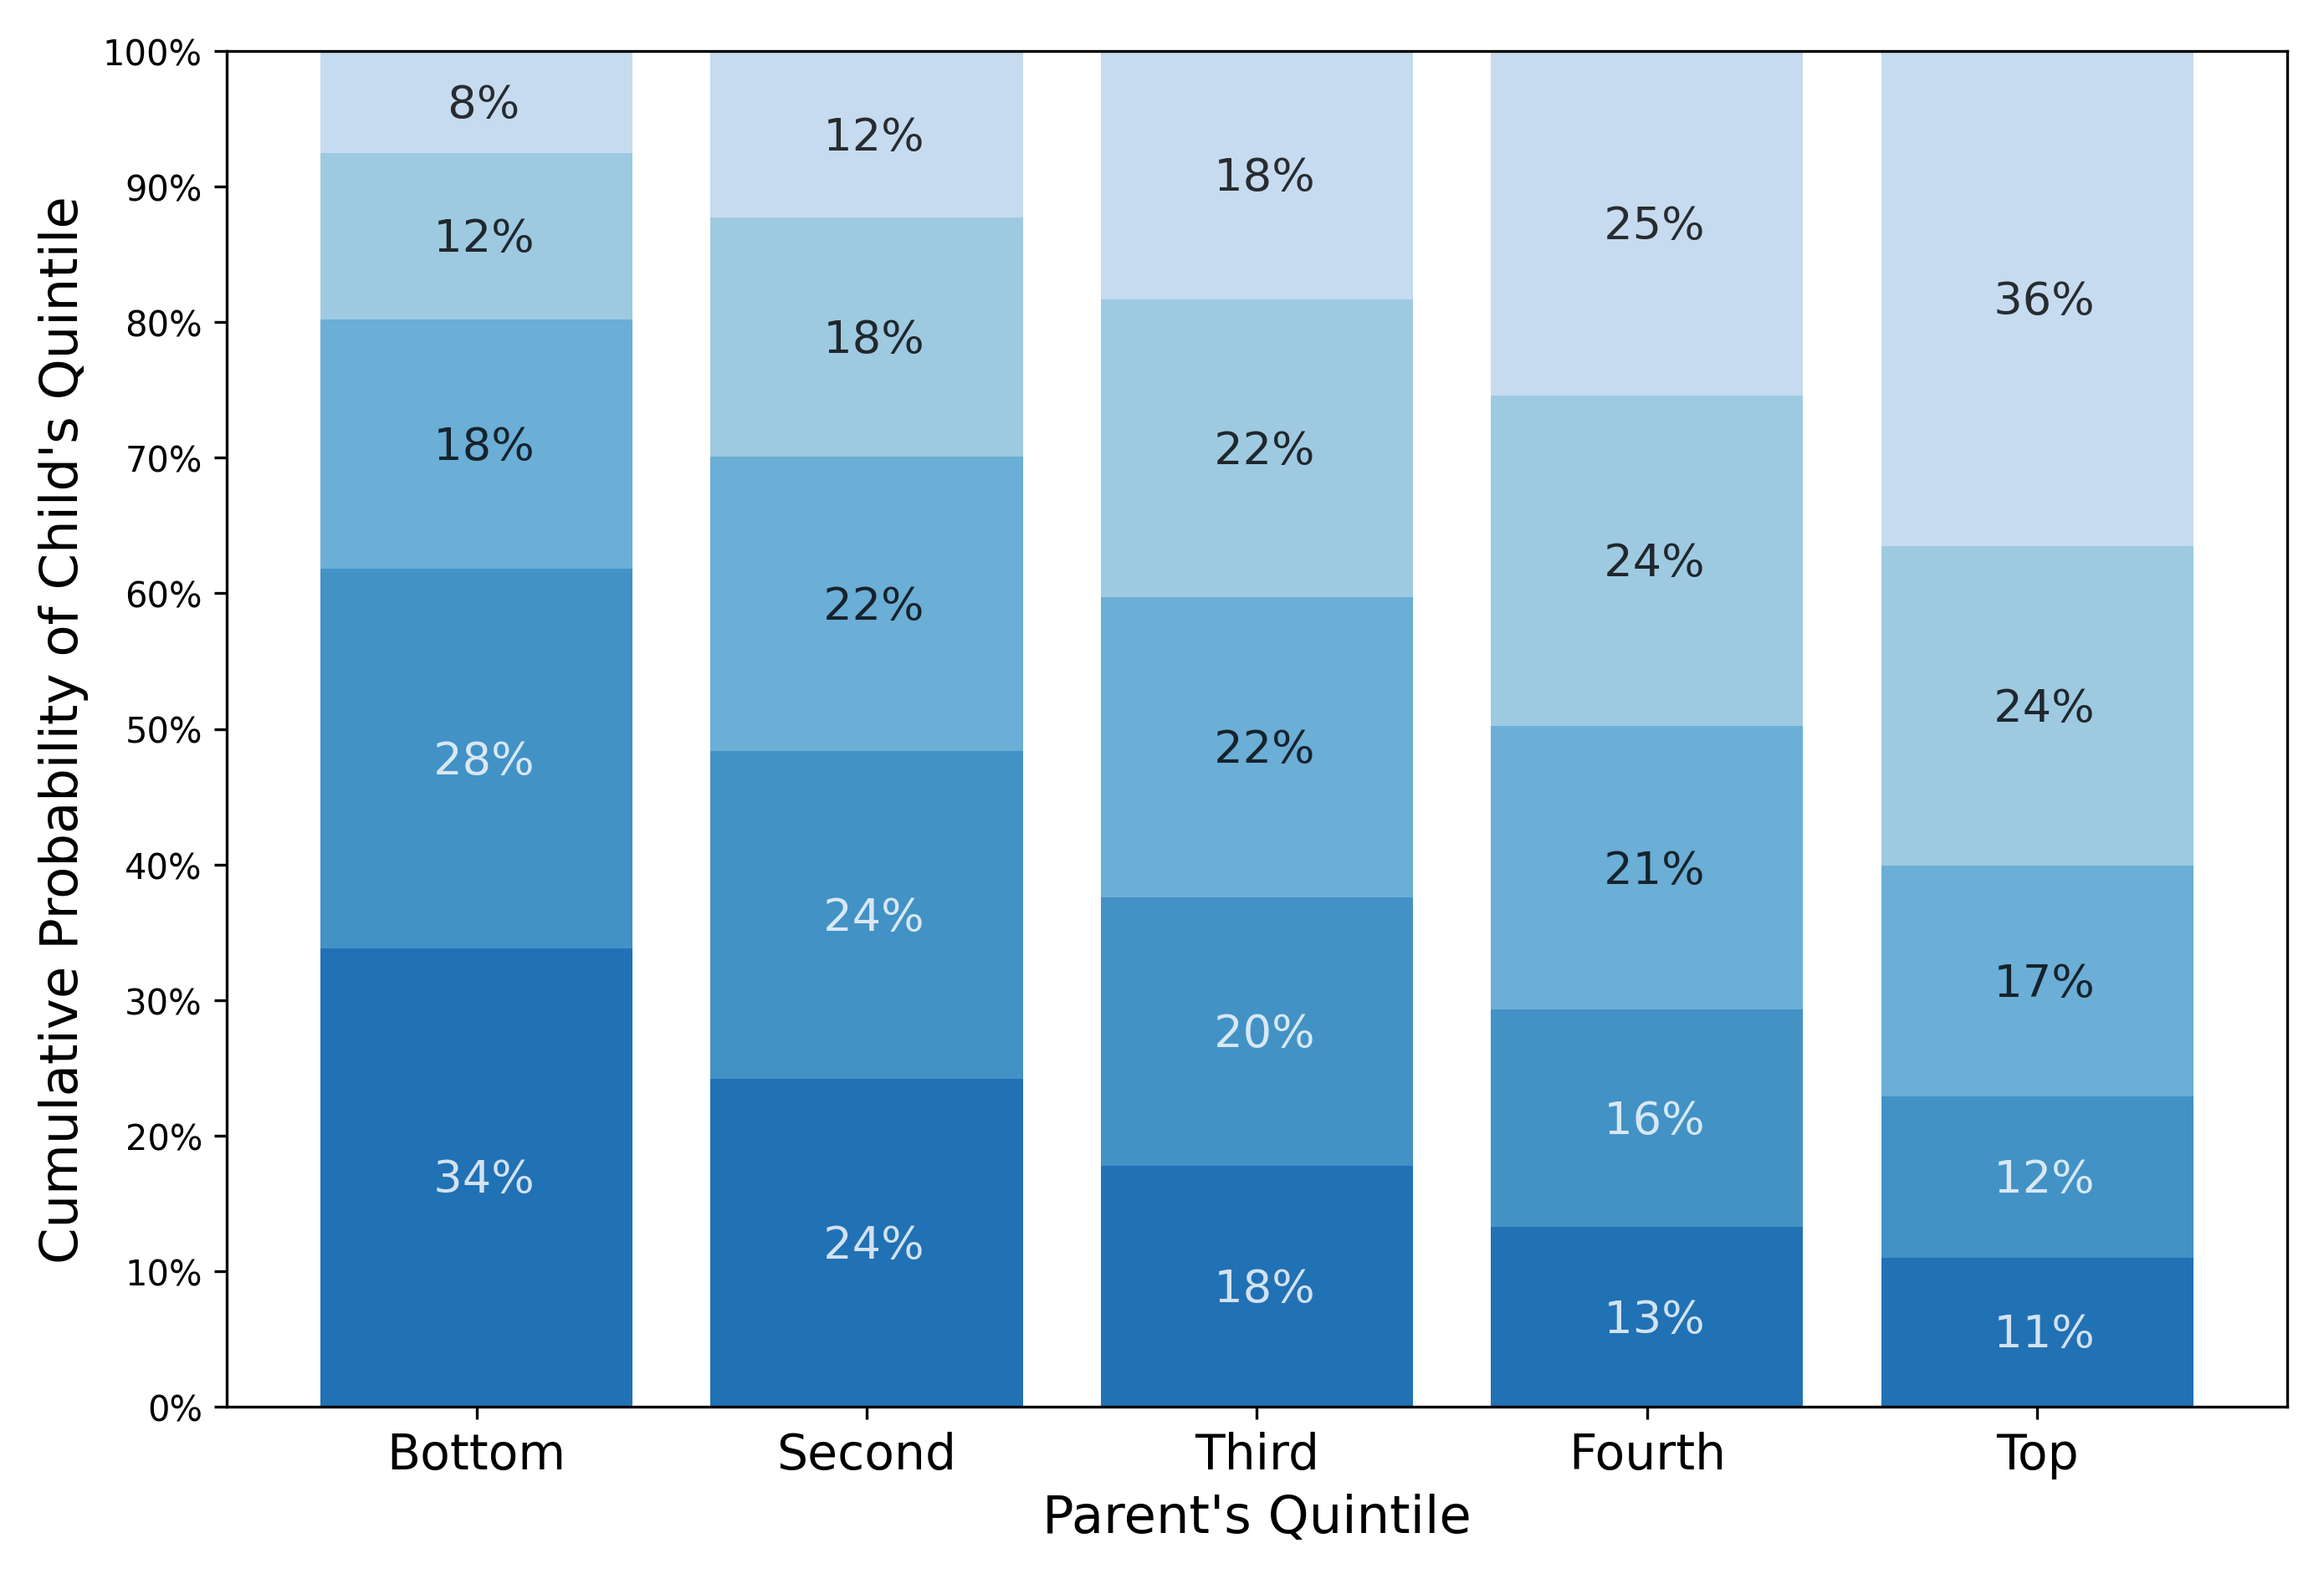
\includegraphics[width=3.5in]{figures/quintile-chetty.png} 
\caption{Parent-to-child quintile transition matrix for US family income data for the 1980-82 birth cohort \cite{chetty}.}
\label{fig:quintile_chetty}
\end{figure}

The heritability of height has been well established, and the similarity between parents and their children can primarily be explained by their shared genealogies \cite{luo, preece, wood}. However, much of the correspondence between the incomes of parents and their children may be reasonably hypothesized to result from environmental factors. Therefore, the income transition matrix suggests the question of whether some of the correspondence between the statures of children and their parents can be explained by environmental factors. Nonetheless, studies of genome-wide SNPs have identified polygenic scores that account for a small amount (~2.5\%) of the variance in family socioeconomic status (SES), including income \cite{trzaskowski, krapohl}. In that case, a normal linear model (and the corresponding Markov process introduced here) may be useful to describe both the genetic \emph{and} environmental factors that relate parents and their children.

%This finding invites a brief discussion on how it might be interpreted. Krapohl and Plomin write that a high degree of heritability in SES is usually interpreted to mean a low degree of social mobility. However, they write that as environmental differences diminish (approaching equal opportunity), individual differences that remain will to a larger proportion be due to genetic differences, increasing the observed heritability. Therefore, the authors posit that the heritability of SES can be viewed as an index of social mobility \cite{trzaskowski, krapohl}.


% DISCUSSION
\section{Discussion}

\subsection{Summary of the model and its important properties}

\subsubsection*{Generalization of the normal linear model}

The model described in this paper extends the normal linear model (linear regression with normally distributed residuals) into a Markov process. The initial state is a normal distribution, and all states after that are also normally distributed. It has immediate application for a polygenic trait such as stature, which is normally distributed, and for which normal linear models have are an established method of predicting adult-child height from parent height.

Normal linear models have previously been applied to the inheritance between parents and children of stature -- a polygenic trait \cite{luo}. Under a linear model, the conditional expectation for a child's score is the weighted average of the parent's score and the mean population score, where the weight of the parent's score is given by the regression coefficient $r$. Around this expectation, or prediction, there is random normal variation with an SD that is assumed in the model to be proportional to the marginal SD of the parent-generation population, where the degree of proportionality is given by the residual coefficient $r_s$. 

This simple formulation relating parents and their children is re-applied through induction as generations reproduce to produce successive generations. The result is a Markov process in discrete time (generations) and continuous space (phenotypic score). From this process, conditional normal distributions are derived for the scores of descendants and ancestors of any generation-gap $n$ apart. Furthermore, the conditional distribution of an ancestor or descendant's score follows an exponential function of convergence to the overall or marginal population distributions as $n$ increases, with rate constants determined by $r$ and $r_s$. In other words, as the distance to a descendant or ancestor increases, prediction-power is lost as an exponential function of the generation-gap. 


\subsubsection*{Marginal population distributions and the stationary distribution}

The simple formulation is also consistent with the overall normal distribution of the polygenic trait in the population. Assuming the parent generation's population is normally distributed, the child generation's population is also normally distributed, as are all descendant and ancestor-generation populations. To obtain the marginal distribution of the child's generation, the rv representing a parent -- scaled by the regression coefficient, is combined additively with the standard normally distributed rv representing the variation about the prediction -- scaled by the residual coefficient. The sum of independent normally distributed rvs is a normal rv with expectation equal to the sum of the expectations and variance equal to the sum of the variances. An immediate result is therefore that the population variance of the child-generation is proportional to that of the parent-generation by $r^2 + r_s^2$. This means that for there to be stable (constant) population variance between generations, $r^2 + r_s^2$ must equal one. 

Stable population variance results in the stationary distribution. That is, the conditional descendant and ancestor distributions are identical for the same generation-gap $n$. Equivalently, the system behaves the same with time going forwards or backward. When scores are indexed by percentile (relative to the population of their generation) there is always time-reversibility (for both stable and unstable population variance). This is because indexing by percentile standardizes the differing population variances of the generations. In other words, the Markov process is always stationary when the scores of descendants and ancestors are indexed by the percentile of their respective generation. 

\subsubsection*{Intergenerational edge persistence}

The model can quantify questions about intergenerational edge persistence. Consider those with scores within an upper or lower edge of the population distribution, for example, the tallest members of the population. To what extent are they the children of parents also within the same edge, and to what extent are they the children of parents in the lower or upper majority (not the edge) of the distribution? (The edge can be defined by having a score above or below some threshold, or having a score within the top or bottom $x$\% of the distribution.) Two general effects have counteracting effects on intergenerational edge persistence: probability and number. That is, parents at the edge of the distribution have a higher probability of having offspring within the same edge-section. However, there are many more parents in the rest of the distribution. The amount of edge persistence thus results from a competition of sorts between the greater probability for the parents at the edge and the greater number of parents with lower probability. Intuitively, when mobility, measured by $m$, is greater, there is less edge persistence and vice versa. 

For example, if the edge is defined as the top 20\% of the distribution, such that being among the \emph{richest} means having a family income in the top 20\%, the question would be: Are the richest people in the US (born between 1980-82) mostly the children of the richest parents or are they primarily from non-rich families (middle class, lower class, etc.)? The answer from Figure \ref{fig:quintile_chetty} is that a majority (64\%) of the richest are the children of parents in the bottom 80\%. That is, the greater number beats the greater probability (for an edge defined as the top 20\%). The greater number also wins for stature at this edge, though to a lesser extent, such that a smaller majority (56\%) of the tallest are the children of parents in the lower four quintiles (see Figure \ref{fig:quintile_pearson}). As the size of the edge gets larger, the percentage from the rest decreases monotonically -- likewise the percentage from within the edge increases. For example, a minority of those in the top 40\% are from parents in the bottom 60\% for both income and stature: 45.5\% and 41\%, respectively. The results for both edge sizes are consistent with the measure of mobility $m$ being greater for income than for stature. 


% USE CASES
\subsection{Use cases of the model}

\subsubsection*{Estimation of parameters}
The regression and residual coefficients provide the SD ratio of the marginal child to the marginal parent-generation population with the following equation:
$$\mathrm{SD}\,\, \mathrm{ratio} =  \sqrt{r^2+r_s^2}$$
Therefore, having estimates of any two of the three values in the above equation means also having an estimate of the third. Likewise, under stable population variance, observing or measuring one of $r$ or $r_s$ immediately gives away the other. When there is stable population variance, $r$ is also the correlation coefficient between parent and child scores and can be estimated that way. Alternatively, the estimates of $r$ and $r_s$ could be obtained by ordinary least squares as shown in this paper. Estimates of $r$ and $r_s$ are sufficient to describe the model.

\subsubsection*{Potential to model both genetic and environmental factors}

The observed approximation of the log-normal distribution to income suggests an application of the model to this domain. That is, a person's income could result from the multiplicative combination of many factors that correlate between parents and children. Then, a person's log-income would be normally distributed due to the central limit theorem, as with stature, and his or her adult-child's log-income could be predicted with a normal linear model.

The example of US family income introduced in the section on visualizations of percentile transition matrices suggests that a normal linear model may be useful to describe the relation between parents and their children for a trait with genetic, or environmental determinants, or a combination thereof. This is especially reasonable to expect if the effects of the environment are also numerous and, on average, small, as are the effects of genes for a polygenic trait. Then, the trait should be normally distributed in the marginal population and fall under the paradigm of the linear model, in which conditional expectation for a child's score is a weighted average (by $r$) of the parent's score and the mean population score. 

In future work, therefore, the Markov process described in this paper could model traits that are approximately normally distributed and for which child scores can be predicted from parent scores with a normal linear model. These traits could have some arbitrary combination of genetic or environmental determinants, as long as they meet those basic two requirements. For such traits, this paper introduces a vocabulary of sorts: the regression coefficient $r$ and the residual coefficient $r_s$, which can be estimated from data (as shown in this paper). Additionally, a justification was made for indicating the amount of mobility, or information-loss, through the ratio of $r_s$ to $r$, given by $m$. Estimates of these terms could enable standard comparisons between such traits, such as the comparisons between stature and income discussed here. 

\subsubsection*{Potential extension to general linear models}

Additional future work could apply the multi-generational extension of the normal linear model shown in this paper to other generalized linear models. This extension was justified for describing a population that reproduces between generations, in which the forward one-step transition between generations is well-modeled by a normal linear relationship. However, other general linear models, such as the Poisson or the Gamma, might also be extended to a Markov process, with potential applications to nature. 

\clearpage


%References


\bibliographystyle{apalike}
\bibliography{polygenic_bib}

\clearpage



% APPENDIX
\section{Appendix}

\subsection{Further mathematical checks}
\subsection*{Verifying the marginal population variance with Eve's law}
We can verify our expression for $\mathrm{Var}(X_{i+n})$ using Eve's law:
%
$$\mathrm{Var}(X_{i+n}) = \mathrm{E}(\mathrm{Var}(X_i|X_{i+n})) + \mathrm{Var}(\mathrm{E}(X_{i+n}|X_i))$$
%
We have separately shown the conditional variance and expectation of the conditional descendant distribution:
%
$$\mathrm{E}(\mathrm{Var}(X_{i+n}|X_i)) = \sigma_i^2 [(r^2+r_s^2)^n-r^{2n}]$$
$$\mathrm{Var}(\mathrm{E}(X_{i+n}|X_i)) = \mathrm{Var}(r^nX_i) = r^{2n}\sigma_i^2$$
%
Combining the terms, we confirm our earlier expression:
%
$$\sigma_{i+n}^2 = (r^2+r_s^2)^n  \sigma_i^2$$

\subsection{Software}
Available at \href{https://github.com/jessebmurray/polygenic}{github.com/jessebmurray/polygenic}

%\ begin{verbatim}

%\end{verbatim}

% Distributed iid: \stackrel{iid}{\sim}

\end{document}



